\documentclass[12pt,letterpaper,titlepage,twoside]{book}
\usepackage[utf8]{inputenc}
\usepackage[spanish]{babel}
\usepackage{amsmath}
\usepackage{amsfonts}
\usepackage{amssymb}
\usepackage[retainorgcmds]{IEEEtrantools}
\usepackage{tikz}
%\usepackage{pstricks}
%\usepackage{auto-pst-pdf}
%\ifpdf
%  \usepackage{tikz}
%\else
%  \usepackage{pst-plot}
%\fi
\usepackage{siunitx}
\usepackage[siunitx]{circuitikz}

\newcommand{\me}{\mathrm{e}}

\author{Alberto Carlos Salas Mier}
\title{Comunicaciones 1 - Notas del Curso}
\begin{document}
\tableofcontents
\chapter{Introducción            (10 Horas)}
\section{Conceptos generales}

\lq \lq Información es poder", reza el dicho. Y en la actualidad como nunca antes, el individuo está ávido de ésta. La demanda de información es tal, que actualmente se está hablando del "Internet de las cosas",concepto según el cual TODO estará conectado a la red. Se pueden ver algunos ejemplos en la actualidad: no somos del todo ajenos a los lentes de google (Google Glass), donde un objeto común está conectado a la Internet, y permite a un usuario del dispositivo obtener información en tiempo real de lugares, tráfico, interacción social entre otros. Recientemente han habido diversos cambio importante relativo a la cantidad de información que se consume: el uso del protocolo Bluetooth es ya masivo; los CDs han sido remplazados por los BD; los celulares comunes fueron desplazados por los denominados Smartphones.
	
Toda esta demanda de información implica necesariamente el diseño de dispositivos que puedan manejarla. Y no únicamente me refiero al almacenaje: los dispositivos deben ser cada vez más pequeños para poderse incorporar dentro de cualquier elemento, mecanismo o aparato común; deben poder también intercambiar información con dispositivos similares o proporcionarla al humano cuando este lo demande. Esto lleva a una rama de la ingeniería en particular: las telecomunicaciones.

El diseño de un sistema de telecomunicaciones es en gran parte un desarrollo tecnológico, pero también es todo un avance científico de la humanidad. Encierra el diseño de circuitos integrados analógicos, la exploración de la teoría de la información, el conocimiento de procesos aleatorios, entre otros. ¿Dónde encaja cada uno de estos elementos? Se deben revisar algunos conceptos esenciales:
\begin{itemize}
\item Señal: Es una cantidad que depende de otra; típicamente se depende del tiempo y regularmente se conoce su valor a partir de una medición. Se representa matemáticamente como una función. 

\item Sistema: Conjunto de elementos que interactúan para obtener un resultado.
\item Comunicación: Proceso de llevar información de un punto a otro.
\end{itemize} 

\textbf{Este curso se centra en el análisis de los dispositivos electrónicos que se requieren para lograr una comunicación inalámbrica efectiva; por lo tanto es requerido un fondo fuerte en circuitos eléctricos y electrónica analógica}

\emph{Proyectos: RDF, SDR, radar...}
  
\section{Perspectiva Histórica}

Resulta curioso que se asocian los sistemas digitales a la tecnología mas reciente, sin embargo con respecto a las telecomunicaciones, primero fueron los sistemas digitales que los analógicos. Uno de los primeros sistemas de telecomunicaciones fue el telégrafo de Morse, quién diseñó un sistema binario para codificar las letras tomando en cuenta la distribución probabilista de los símbolos que componen el alfabeto. Esto ocurría en 1837 y para 1844, ya se tenía un sistema completamente operativo.

Las comunicaciones inalámbricas se basan en los desarrollos de Hertz, Oersted, Maxwell, Faraday, entre otros. Oersted demostró que una corriente que circula por un conductor produce un campo magnético y Faraday la inducción: un campo magnético que cambia produce una corriente en un conductor cercano. En 1864, James C. Maxwell predijo la radiación electromagnética y formuló la teoría básica; sus resultados fueron comprobados experimentalmente por Hertz en 1887.

Se le da el crédito a Marconi del desarrollo de la telegrafía sin hilos; el demostró la transmisión de señales de radio a dos kilómetros de distancia en 1895.En 1901 se realizó la primera transmisión transatlántica.

La invención del tubo de vacío permitió el desarrollo de la radio comercial en la primera parte del siglo XX. La transmisión en AM inició en 1920. Armstrong desarrolló el esquema superheterodino y la FM. Hacia 1933 demostró su utilidad pero no se desarrolló comercialmente hasta el fin de la segunda guerra mundial.

En 1929  se desarrolló el primer sistema de televisión y en Gran Bretaña comenzó el sistema de difusión en 1936. 

En la segunda mitad del siglo XX, el desarrollo del transistor por Shockley, Bardeen y Brattain, y el circuito integrado por Kilby	y Noyce, permitieron la construcción de dispositivos más pequeños, con menos consumo de energía y más veloces que hicieron posible el crecimiento de los sistemas de comunicación con satélites y fibra óptica.

Actualmente la demanda de datos crece a ritmos espectaculares: la telefonía celular, los sistemas de percepción remota y la llegada del internet de las cosas (IoT) hacen que estemos en los albores de una nueva era de comunicaciones. 

\section{Modulación y Demodulación}

Realice un experimento rápido: tome una hoja de papel, y tal como está, intente hacerla llegar lo más lejos posible. Ahora forme una bola con ella y pruebe de nuevo. Ahora toma una piedra pequeña y envuélvala con el papel. Qué ocurrió? Eso ilustra el objetivo de la modulación: permitir que algo aproveche las características del medio para llegar más lejos. En el caso de las comunicaciones electrónicas, lo que se debe enviar es la información, la cual adopta el formato de un mensaje quién a su vez es convertido a señales eléctricas. 
%Se ha demostrado (y ese no es el objetivo de este material) que éste tipo de señales

Como en el caso del papel, el medio permite o limita la capacidad de transmisión de las señales eléctricas (o radiación electromagnética, para ser más precisos). Por lo tanto también se debe realizar un proceso equivalente, es decir, acoplar la señal al medio; éste es el objetivo de la modulación.

En el caso particular las señales electromagnéticas deben ser acondicionadas para transmitirlas eficientemente por el aire o por un conductor. Es necesario conocer los conceptos de espectro y ancho de banda para ilustrar el efecto de modulación, sin embargo el concepto es más sencillo: la modulación consiste en modificar los parámetros (amplitud, frecuencia, fase) de una señal. Y el nombre del tipo de modulación depende de esto, es decir: si se modifica la amplitud, es amplitud modulada, si se modifica la frecuencia es frecuencia modulada y si se modifica la fase es fase modulada. Es necesario introducir tres conceptos nuevos: señal portadora, señal moduladora y señal modulada.

\begin{itemize}
\item La señal portadora es el equivalente a la piedra,es decir, es el vehículo que permite que el objeto que deseamos transmitir llegue más lejos; es una señal de alta frecuencia que puede viajar mejor por el aire. Son los parámetros de esta señal los que se modifican. La frecuencia de portadora está determinada por la factibilidad de implementación: la construcción de antenas y transmisores depende de esta cantidad.
\item La señal moduladora es la señal de información, comunmente referida como banda base, y es típicamente de baja frecuencia; los parámetros de la portadora se modifican  normalmente en proporción lineal a la amplitud de este valor.
\item La señal modulada es la señal que resulta de la modulación; obsérvese que se trata de una nueva señal con características diferentes a las dos anteriores.
\end{itemize}

Posteriormente se detallará cómo se realiza el proceso de modulación, los  dispositivos que intervienen en ella y qué consecuencias tiene.

La demodulación es el proceso inverso, es decir, recuperar la señal moduladora de la señal modulada. 




\section{El espectro Electromagnético}

Las comunicaciones electrónicas utilizan señales electromagnéticas para transmitir los mensajes a través del espacio. Estas señales se caracterizan por ser dos señales ortogonales entre sí, una de campo eléctrico y otra de campo magnético. Se ilustra en la Figura \ref{wave}.

\begin{figure}[th]
\begin{center}
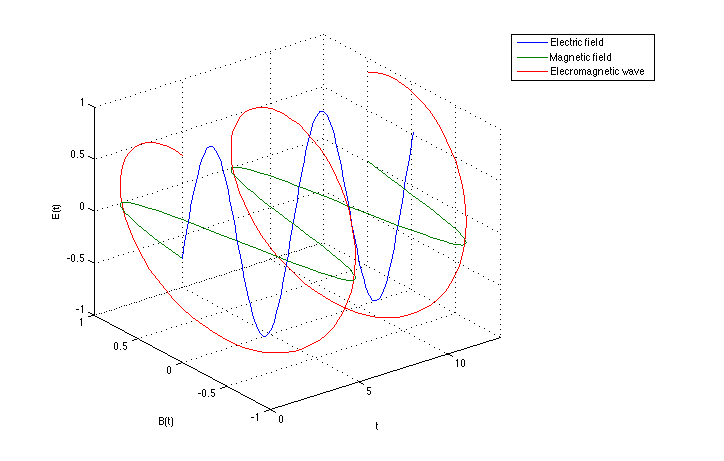
\includegraphics[scale=.7]{./wave.png}\caption{Onda Electromagnética.}\label{wave}
\end{center}
\end{figure} 

Esta onda, que tiene la propiedad de interactuar con la materia, viaja a la velocidad de la luz y presenta dos propiedades de vital importancia para el análisis y diseño de sistemas de comunicaciones electrónicas: frecuencia y longitud de onda, las cuales se relacionan por medio de la Ecuación \ref{longfrec}
\begin{equation}
f = c/\lambda 
\end{equation}
donde $f$ es frecuencia en Hertz, $c$ es la constante de la velocidad de la luz en metros sobre segundo y $\lambda$ es longitud de onda en metros.

El espectro electromagnético incluye las frecuencias desde milésimas de Hertz hasta varios Terahertz.


\subsection{Frecuencias de Transmisión}

%más información de Parsons : Mobile radio propagation channel
El espectro electromagnético se divide en bandas o regiones de frecuencia, y se asignan para un uso en particular. Este uso particular puede ser transmisión comercial de radio y televisión o uso reservado por el ejército. Suele ocurrir que bandas previamente asignadas sean destinadas a otro uso; también existen las bandas "libres", entre las que destacan las bandas ISM y las de radio amateur. Comercialmente se tienen las siguientes bandas asignadas: 

\begin{itemize}
\item AM : 500 – 1500 kHz
\item FM : 88 – 108 MHz
\item ISM : 860 MHz, 915 MHz, 2.4 GHz
\item Radar : mmw  30GHz
\end{itemize}

Una clasificación más general, y que además es establecida por la ITU, se muestra a continuación:



\begin{tabular}{|c|c|}
\hline 
300 - 3000 kHz & MF \\ 
\hline 
3 - 30 MHz & HF \\ 
\hline 
30 -  300 MHz & VHF \\ 
\hline 
.3 - 3 GHz & UHF \\ 
\hline 
\end{tabular} 

Pregunta: qué implica el uso de bandas? 
Longitud de onda: $\lambda = c/f$
\textbf{Por dónde se propaga la onda}

\emph{Las condiciones de propagación dependen de la frecuencia.}  Existen básicamente 3 tipos de propagación: onda terrestre, onda celeste y línea de vista. Abajo de 2 MHz, es onda terrestre. Las características de propagación resultan de los cambios en la velocidad de las ondas de radio como una función de la altitud y las condiciones limitantes. La velocidad de la onda depende de la temperatura aerea, la densidad del aire y los niveles de ionización aereos.

\begin{itemize}
\item La transformación de la señal primaria a una señal adecuada para ser enviada por el sistema de radiocomunicaciones se realiza por medio del bloque del modulador. 
\item El transmisor centra la información en una frecuencia particular (bloque del modulador) y la transforma en señales con energía electromagnética (bloque transceptor de energia). 
\end{itemize}

Cuáles son los criterios para decidir qué frecuencia utilizar?

\subsection{Clasificación de Transmisores (Eliminado - corresponde a USA)}



\subsection{Ancho de Banda y Capacidad de información}

Una de las preguntas fundamentales es ¿Cuanta información podemos enviar por un canal?

Existen dos condiciones: sistemas analógicos y sistemas digitales; tomando en cuenta que los dos mecanismos que se inciden en la calidad del enlace son la potencia de transmisión y el ruido del canal, se busca tener un sistema que, en el caso digital, minimice la probabilidad de bit erroneo sujeto a aquellas restricciones; en el caso analógico, que maximice la relación entre la potencia de la señal y la potencia del ruido a la salida del receptor. Es necesario comprender un concepto fundamental:

Definición de Ancho de banda: es el contenido frecuencial de una señal

¿Cómo se relaciona el ancho de banda con la cantidad de información que es posible enviar a través de un enlace?

En 1949, C.E. Shannon, en un articulo fundamental, definió que para cierto canal  de ancho de banda $B$ y potencia de señal $S$ y de ruido $N$, se puede enviar un maximo de 
\begin{equation}
C = B \log_2 \left( 1+\frac{S}{N} \right) 
\end{equation}

lo que implica que si la fuente genera información por debajo de este valor, se puede lograr una tasa de bit erroneo cercana a cero.
%¿Cuáles son las limitaciones fundamentales de la transmisión de información

\subsection{Organismos Legales que regulan la Utilización del espectro}

En México, la regulación de telecomunicaciones la realizan tanto la Secretaría de Comunicaciones y Transportes y la Comisión Federal de Telecomunicaciones.

Del Instituto, según lo marca la Ley Federal de Telecomunicaciones y Radiodifusión, se menciona que 
\begin{itemize}
\item El Instituto es un  órgano público autónomo, independiente en sus decisiones y funcionamiento, con personalidad jurídica y patrimonio propios, que tiene por objeto regular y promover la competencia y el desarrollo eficiente de las telecomunicaciones y la radiodifusión en el ámbito de las atribuciones que le confieren la Constitución y en los términos que fijan esta Ley y demás disposiciones legales aplicables. 

El Instituto tiene a su cargo la regulación, promoción y supervision del uso, aprovechamiento y explotación del espectro radioeléctrico, los recursos orbitales, los servicios satelitales, las redes publicas de telecomunicaciones y la prestación de los servicios de radiodifusión y de telecomunicaciones, así como del acceso a la infraestructura activa y pasiva y otros insumos esenciales, sin perjuicio de las atribuciones que corresponden a otras autoridades en los términos de la legislación correspondiente.

Asimismo, el Instituto es la autoridad en materia de competencia económica de los sectores de radiodifusión y telecomunicaciones, por lo que en éstos ejercerá en forma exclusiva las facultades que establecen el articulo 28 de la Constitución, esta Ley y la Ley Federal de Competencia Económica.
El Instituto es la autoridad en materia de lineamientos técnicos relativos a la infraestructura y los equipos que se conecten a las redes de telecomunicaciones, así como en materia de homologacion y evaluación de la conformidad de dicha infraestructura y equipos."
\end{itemize}

A la Secretaría, corresponde, entre muchos otros:

\begin{itemize}
\item Emitir opinión técnica no vinculante al Instituto, en un plazo no mayor a treinta días naturales sobre el otorgamiento, la prórroga, la revocación, así como la autorización de cesiones o cambios de control accionario, titularidad u operación de sociedades relacionadas con concesiones en materia de telecomunicaciones y radiodifusión;
\item Planear, fijar, instrumentar y conducir las políticas y programas de cobertura universal y cobertura social de conformidad con lo establecido en esta Ley;
\item Elaborar las políticas de telecomunicaciones y radiodifusión del Gobierno Federal.
\end{itemize}


En el ámbito internacional, corresponde a la Unión Internacional de Telecomunicaciones: La UIT es el organismo especializado de las Naciones
Unidas para las tecnologías de la información y la
comunicación (TIC). Como tal, es responsable de la
atribución del espectro de frecuencias radioeléctricas
y las órbitas de satélite, y de la normalizacion y
el desarrollo de las TIC en el mundo. La UIT se ha
comprometido con determinación a conectar a todos
los habitantes del mundo, independientemente de su
lugar de residencia y de sus recursos, y a proteger el
derecho fundamental de todos a comunicar.


Ojo con los artículos 189 y 190 de la LFTyR
\section{Repaso de Análisis de señales}

Ejemplos de señal
¿Qué se entiende por señal?
Clasificación y Ejemplo de señales
Señales sinusoidales (representación en tiempo y frecuencia)

Frecuencia fundamental y armónicas
Serie de Fourier para una onda rectangular
El espectro de potencia y el espectro de Energía
Efecto de Limitación de Banda sobre las señales


\subsection{Señales Senoidales}
Una señal periódica es aquella que se repite cada cierto tiempo;matemáticamente, $f(t)$ es periódica sí:

\begin{equation}
f(t)  = f(t+T)
\end{equation}

donde $T$ es el período de la señal.

Las funciones periódicas son caracterizadas  por tres parámetros: amplitud, frecuencia y fase, mostrado en la Figura \ref{senal} . 

\begin{figure}
\begin{center}
\ifx\du\undefined
  \newlength{\du}
\fi
\setlength{\du}{15\unitlength}
\begin{tikzpicture}[domain=0:3, scale=3]
\draw[very thin,color=gray] (-0.1,-1.1) grid (2.9,1.9);
\draw[arrows = ->] (-0.2,0) -- (4.2,0) node[right] {$x$};
\draw[arrows = ->] (0,-1.2) -- (0,2.2) node[above]{$f(x)$};
\draw[arrows = <->]  (0,-1.30) -- (1,-1.3) node[fill=white,inner sep=1pt] at (.5,-1.3){$T = \frac{1}{f}$}; 
\draw  (.250,0) -- (.25,.7) ; 
\draw[arrows = <->]  (0,.7) -- (.25,.7) node[fill=white,inner sep=1pt] at (.125,.7){$\phi$}; 
\draw[color=blue, samples = 6500] plot[id=sin] function{sin(pi*2*x-pi/2)} node[above] at(2.5,1) {$A$}; 

\end{tikzpicture}
\end{center}
\caption{Parámetros de una señal}\label{senal}
\end{figure}

Problema: 
Encontrar el período de la función 

Un tipo especial de señales periódicas lo constituyen las señales sinusoidales. Este tipo de funciones simples se utilizan para representar otro tipo de funciones más complejas, como a señal cuadrada, triangular, etc...



\subsection{Series de Fourier}

\subsubsection{Ortogonalidad}
La teoría de álgebra lineal indica que un par de vectores son ortogonales si y solo si su producto interno (o producto escalar) es igual a 0. Los conceptos de campo vectorial se puede extender a funciones para tener campos de funciones, lo que proporciona la extensión del concepto de ortogonalidad a espacios de señales; es decir, una señal se puede representar como una combinación lineal de funciones base, o que se tiene una representación para la señal relativa a tal base.

Se elige las funciones seno y coseno dado que son funciones ortogonales (entre sí).
Demostración: 
Se define que el producto interno entre dos funciones $f(x)$ y $g(x)$ está dada por 
\begin{equation}
\left( x,y \right) = \int_T x(t) y^*(t) dt; \
\end{equation}

Si se elige las funciones $f(x) = \sin n \omega_0 t$ y $f(x) = \cos n \omega_0 t$ se tiene que 

\begin{equation}
\int \sin n \omega_0 t \cos m\omega_0 t dt
\end{equation}

Por identidades trigonométricas, 
\begin{equation}
\sin \left( \alpha + \beta \right) = \sin \alpha \cos \beta + \sin \beta \cos \alpha
\end{equation}

\begin{equation}
\int \sin n \omega_0 t \cos m\omega_0 t dt = \int \sin  \left( n \omega_0 t + m\omega_0 t \right) + \sin  \left( n \omega_0 t - m\omega_0 t \right) dt
\end{equation}



\textbf{Ejercicio:}

\textit{Demuestre que tanto la onda coseno como la onda seno son ortogonales consigo mismas para frecuencias armónicas.}

\subsubsection{La base de Fourier}

Una señal periódica puede descomponerse en una sumatoria de señales seno y coseno.  Este procedimiento es conocido como \emph{análisis}; el procedimiento inverso, es decir, formar una señal periódica a partir de señales seno y coseno, se conoce como síntesis. 
Entonces:
\begin{align}
f(t)  &=\frac{1}{2}a_0+a_1 \cos \omega_0 t +a_2 \cos 2 \omega_0 t + \cdots + b_1 \sin \omega_0 t + b_2 \sin 2\omega_0 t + \cdots \nonumber \\
&= \frac{1}{2}a_0 + \sum_{n=1}^\infty a_n \cos n \omega_0 t+ b_n \sin n \omega_0 t \label{trigdefourier}
\end{align}

con $\omega_0 = \frac{2 \pi}{T}$. Esta es conocida como la serie trigonométrica de Fourier.

\begin{equation}
f(t) = C_0 + \sum C_n \cos \left(n \omega_0 t - \theta_n \right)
\end{equation}

La componente sinusoidal  de frecuencia $\omega_n = n\omega_0$ se denomina la $n$-ésima armónica de la función periódica. La primera armónica se conoce comunmente como la componente fundamental.



Utilizando las relaciones de ortogonalidad, se pueden evaluar los coeficientes de la serie de Fourier. Comenzamos con la ec. \ref{trigdefourier}

\begin{equation*}
f(t) = \frac{1}{2}a_0 + \sum_{n=1}^\infty a_n \cos n \omega_0 t+ b_n \sin n \omega_0 t
\end{equation*}

Si se multiplica ambos lados por $\cos m \omega_0 t$ e integrando entre $\left[ -T/2  \right]$ y $\left[- T/2 \right]$



\begin{IEEEeqnarray}{rCl} 
\int^{T/2}_{-T/2} f(t) \cos m \omega_0 t dt &=&\frac{a_0}{2} \int^{T/2}_{-T/2} \cos m \omega_0 t dt + \int^{T/2}_{-T/2} \sum_{n = 1}^{\infty} a_n \cos n \omega_0 t\cos m \omega_0 t dt \nonumber\\ && +\: \int^{T/2}_{-T/2} \sum_{n = 1}^{\infty}b_n  \sin n \omega_0 t\cos m \omega_0 t dt  
\end{IEEEeqnarray}

esto es:

\begin{IEEEeqnarray}{rCl} 
\int^{T/2}_{-T/2} f(t) \cos m \omega_0 t dt &=&\frac{a_0}{2} \int^{T/2}_{-T/2} \cos m \omega_0 t dt + \sum_{n = 1}^{\infty} a_n\int^{T/2}_{-T/2}  \cos n \omega_0 t\cos m \omega_0 t dt \nonumber\\ && +\: \sum_{n = 1}^{\infty}b_n\int^{T/2}_{-T/2}   \sin n \omega_0 t\cos m \omega_0 t dt  
\end{IEEEeqnarray}

Aplicando los resultados de la ortogonalidad, se tiene que

\begin{equation}
a_n = \frac{2}{T} \int_{-T/2} ^{T/2} f(t) \cos m\omega_0 t dt
\end{equation}

 \emph{Se dewjará al estudiante que demuestre los coeficientes $b_n$ y $a_0$}
 
 
Si a la misma Ecuación \ref{trigdefourier} ahora se integra entre $\left[ -T/2  \right]$ y $\left[- T/2 \right]$ se tiene

se tiene 

\begin{equation}
 a_0 = \frac{2}{T}\int_{-T/2}^{T/2} f(t) dt
  \end{equation} 

Finalmente, para obtener los coeficientes $b_m$:

Si se multiplica ambos lados por $\sin m \omega_0 t$ e integrando entre $\left[ -T/2  \right]$ y $\left[- T/2 \right]$



\begin{IEEEeqnarray}{rCl} 
\int^{T/2}_{-T/2} f(t) \sin m \omega_0 t dt &=&\frac{a_0}{2} \int^{T/2}_{-T/2} \sin m \omega_0 t dt + \int^{T/2}_{-T/2} \sum_{n = 1}^{\infty} a_n \cos n \omega_0 t\sin m \omega_0 t dt \nonumber\\ && +\: \int^{T/2}_{-T/2} \sum_{n = 1}^{\infty}b_n  \sin n \omega_0 t\sin m \omega_0 t dt  
\end{IEEEeqnarray}

esto es:

\begin{IEEEeqnarray}{rCl} 
\int^{T/2}_{-T/2} f(t) \cos m \omega_0 t dt &=&\frac{a_0}{2} \int^{T/2}_{-T/2} \cos m \omega_0 t dt + \sum_{n = 1}^{\infty} a_n\int^{T/2}_{-T/2}  \cos n \omega_0 t\cos m \omega_0 t dt \nonumber\\ && +\: \sum_{n = 1}^{\infty}b_n\int^{T/2}_{-T/2}   \sin n \omega_0 t\cos m \omega_0 t dt  
\end{IEEEeqnarray}

Aplicando los resultados de la ortogonalidad, se tiene que

\begin{equation}
b_n = \frac{2}{T} \int_{-T/2} ^{T/2} f(t) \sin m\omega_0 t dt
\end{equation}




\subsection{Serie de Fourier para una onda rectangular}

\emph{Este subtema lo podrían resolver los alumnos como ejercicio de clase; se añade para referencia}

\begin{IEEEeqnarray*}{rcl} 
a_n &=& \int^{T/2}_{-T/2} f(t) \cos n \omega_0 t dt =\frac{2}{T} \left( \int^{0}_{-T/2} - \cos n \omega_0 t dt + \int^{T/2}_{0}  \cos n \omega_0 t dt \right) \nonumber\\ &=&  \frac{2}{T} \left( \left. - \frac{1}{n \omega_0}  \sin n \omega_0 t \right\vert_{- \frac{T}{2}}^{0}  + \left. \frac{1}{n \omega_0}  \sin n \omega_0 t \right\vert_{0}^{ \frac{T}{2}}   \right) \nonumber\\ 
&=& \frac{2}{T} \left\lbrace -\frac{1}{n \omega_0}  \left[ \sin 0 - \sin \left( - n \omega_0 \frac{T}{2} \right)   \right] + \frac{1}{n \omega_0}  \left[ \sin 0 - \sin \left( - n \omega_0 \frac{T}{2} \right)   \right] \right\rbrace \nonumber \\
&=& 0 \nonumber
\end{IEEEeqnarray*}


\begin{IEEEeqnarray*}{rcl} 
b_n &=& \int^{T/2}_{-T/2} f(t) \sin n \omega_0 t dt =\frac{2}{T} \left( \int^{0}_{-T/2}-\sin n \omega_0 t dt + \int^{T/2}_{0}  \sin n \omega_0 t dt \right) \nonumber\\ &=&  \frac{2}{T} \left( \left.  \frac{1}{n \omega_0}  \cos n \omega_0 t \right\vert_{- \frac{T}{2}}^{0}  - \left. \frac{1}{n \omega_0}  \cos n \omega_0 t \right\vert_{0}^{ \frac{T}{2}}   \right) \nonumber\\ 
&=& \frac{2}{n \omega_0 T} \left\lbrace  \left[ 1 - \cos \left( n \omega_0 \frac{T}{2} \right)   \right] -  \left[ \cos \left( - n \omega_0 \frac{T}{2} \right) -1  \right] \right\rbrace \nonumber \\
&=& \frac{2}{n\pi} \left( 1 - \cos n\pi \right) = \frac{2}{n\pi}  \left[ 1-\left( -1 \right)^n \right] \nonumber
\end{IEEEeqnarray*}

\subsection{El espectro de potencia y de energía}

El contenido de potencia de una función periódica $f(t)$ está definido como el valor cuadrático medio 
\begin{equation}
P = \frac{1}{T} \int_{-\frac{T}{2}}^{\frac{T}{2}} \left[ f \left( t \right)\right]^2 dt \label{eq:pot}
\end{equation}

Si se supone que $f(t)$ es una onda de voltaje o corriente, la ecuación \ref{eq:pot} representa la potencia entregada por la señal a una resistencia de $1 \Omega$.

\emph{Pregunta: Qué es una señal de potencia y qué es una señal de energía?  Es conveniente hacer una introducción en el sentido de que para sistemas de comunicación digitales, es conveniente tratar con señales de energía}


\subsection{Efecto de la limitación de banda sobre las señales}

Al obtener el espectro de una señal que existe para todo $t$, se puede observar que éste existe para una cantidad discreta de valores en frecuencia; por el contrario, una señal que sólo existe para un valor finito de tiempo, se observará que el espectro se vuelve continuo. Se dice entonces que una señal limitada en tiempo es ilimitada en frecuencia, y una señal limitada en frecuencia es ilimitada en tiempo.

Se proporcionan las siguientes definiciones: 

\begin{itemize}
\item Una forma de onda $w(t)$ es absolutamente \textit{limitada en banda }a $B$  hertz si
\begin{equation}
W(f) = \mathcal{F} \left[ w(t) \right] = 0, \; \text{para} \; \vert f \vert  \geqslant B
\end{equation}
\item Una forma de onda $w(t)$ es absolutamente \textit{limitada en tiempo } si
\begin{equation}
w(t) = 0, \; \text{para} \; \vert t \vert  > T
\end{equation}

\end{itemize}

de lo que se desprende el siguiente teorema:

\emph{Una forma de onda absolutamente limitada en banda no puede ser absolutamente limitada en tiempo y viceversa}

% de Carlson:

Obsérvese el comportamiento en la salida de un filtro pasabajas ideal: en frecuencia, la salida está limitada en banda, pero en el tiempo es un pulso sinc (revisar) que permanece todo el tiempo.

Cuál es el compromiso de estas observaciones? Si bien se podría pensar que se deben abandonar los modelos de filtros ideales se debe asumir que las señales tienen una caducidad específica.

La solución, en la práctica, es asumir que las señales son limitadas en banda y frecuencia al mismo tiempo. ¿Cómo? Se puede asumir que para intervalos particulares de tiempo  y para alguna frecuencia umbral la señal es despreciable (no hay pérdida de información)

\section{Ruido Eléctrico}
La señal de ruido es en principio de la misma naturaleza que la señal de información, por lo que ...

Existen muchas causas por las que la señal transmitida sufre perturbaciones. Estas se pueden clasificar por distorsión o interferencia.

Distorsión lineal: ocurre debido a cambios del ancho de banda de la señal; puede ser provocada por los retardos de propagación de la señal.

Distorsión no lineal, que ocurre cuando la señal pasa a través de dispositivos no lineales.

Dependiendo de la fuente, la distorsión puede ser determinista o estocástica.

Entre estas perturbaciones se debe analizar con particular cuidado las interferencias.
Se puede tener la siguiente clasificación de las perturbaciones

Interferencias externas: fenómenos cósmicos, atmosféricos, climáticos, y sistemas de comunicación adyacentes.
Interferencias internas: debidos a defectos en la construcción de dispositivos y al inherente movimiento electrónico.

Esta clase de perturbación es siempre estocástica.



\subsection{Ruido no correlacionado}
Tomasi: Es ruido que está presente independientemente de que exista señal o no. Se puede clasificar en ruido externo y ruido interno.
El ruido externo se genera fuera del dispositivo: atmosférico, extraterrestre o causado por el hombre.

El ruido interno se genera al interior de los dispositivos: ruido de disparo, ruido de tiempo de tránsito y ruido térmico.

\subsection{Ruido correlacionado}
Tomasi: Ruido que depende de la señal; se puede interpretar con la frase "Hay señal. hay ruido"
Se produce por amplificación no lineal: distorsión por intermodulación y distorsión armónica. 
%la distorsión Couch: 251

Qué es un sistema lineal ?

Principio de superposición: 
La respuesta completa de un sistema a un conjunto de entradas es la suma de la respuesta a cada entrada individual:

\begin{equation}
\mathcal{L}\left\lbrace aX_1+bX_2\right\rbrace = a\mathcal{L}\left\lbrace X_1\right\rbrace +b\mathcal{L}\left\lbrace X_2\right\rbrace 
\end{equation}

¿Qué ocurre cuando un amplificador es trabajado más allá de su voltaje de polarización?

La respuesta de un amplificador que incluye la región de saturación se modela más adecuadamente utilizando una serie de Taylor (al rededor de $v_i = 0$); así, la relación entrada -  salida es
\begin{equation}
v_o = K_0+K_1 v_i+K_2 v_i^2+ \cdots = \sum_{n=0}^\infty K_n v_i^n
\end{equation}

donde 
\begin{equation}
K_n = \frac{1}{n!}\left( \frac{d^n v_o}{•} \right)
\end{equation}
Ejercicio: 


\subsection{Relación señal a ruido}
El cociente entre la potencia de la señal y la potencia del ruido
\subsection{Factor de Ruido e indice de ruido o Figura de ruido}
%de Couch 582 -> 586

\section{Generación de Señales}

Los esquemas de modulación requieren la modificación de un parámetro de una portadora de alta frecuencia para permitir la transmisión de manera adecuada. Esto significa que hay que construir esta señal. La señal debe mantener oscilaciones estables para poder ser usada como portadora. Los circuitos que realizan esta función se les conoce como osciladores y se basan en el concepto de retroalimentación positiva. La figura \ref{fig:fb} ilustra este concepto.
\begin{figure}
% Graphic for TeX using PGF
% Title: /Users/Terri/Documents/FIE/Com 1/latex/feedback.dia
% Creator: Dia v0.97.2
% CreationDate: Mon Aug  4 11:53:42 2014
% For: Terri
% \usepackage{tikz}
% The following commands are not supported in PSTricks at present
% We define them conditionally, so when they are implemented,
% this pgf file will use them.
\ifx\du\undefined
  \newlength{\du}
\fi
\setlength{\du}{15\unitlength}
\begin{tikzpicture}[scale = 3]
\pgftransformxscale{1.000000}
\pgftransformyscale{-1.000000}
\definecolor{dialinecolor}{rgb}{0.000000, 0.000000, 0.000000}
\pgfsetstrokecolor{dialinecolor}
\definecolor{dialinecolor}{rgb}{1.000000, 1.000000, 1.000000}
\pgfsetfillcolor{dialinecolor}
\definecolor{dialinecolor}{rgb}{1.000000, 1.000000, 1.000000}
\pgfsetfillcolor{dialinecolor}
\pgfpathellipse{\pgfpoint{2.700000\du}{0.900000\du}}{\pgfpoint{0.900000\du}{0\du}}{\pgfpoint{0\du}{0.900000\du}}
\pgfusepath{fill}
\pgfsetlinewidth{0.000000\du}
\pgfsetdash{}{0pt}
\pgfsetdash{}{0pt}
\pgfsetmiterjoin
\definecolor{dialinecolor}{rgb}{0.000000, 0.000000, 0.000000}
\pgfsetstrokecolor{dialinecolor}
\pgfpathellipse{\pgfpoint{2.700000\du}{0.900000\du}}{\pgfpoint{0.900000\du}{0\du}}{\pgfpoint{0\du}{0.900000\du}}
\pgfusepath{stroke}
% setfont left to latex
\definecolor{dialinecolor}{rgb}{0.000000, 0.000000, 0.000000}
\pgfsetstrokecolor{dialinecolor}
\node at (2.700000\du,1.095000\du){};
\pgfsetlinewidth{0.000000\du}
\pgfsetdash{}{0pt}
\pgfsetdash{}{0pt}
\pgfsetbuttcap
{
\definecolor{dialinecolor}{rgb}{0.000000, 0.000000, 0.000000}
\pgfsetfillcolor{dialinecolor}
% was here!!!
\pgfsetarrowsend{stealth}
\definecolor{dialinecolor}{rgb}{0.000000, 0.000000, 0.000000}
\pgfsetstrokecolor{dialinecolor}
\draw (0.000000\du,0.896552\du)--(1.800000\du,0.900000\du);
}
\pgfsetlinewidth{0.000000\du}
\pgfsetdash{}{0pt}
\pgfsetdash{}{0pt}
\pgfsetbuttcap
{
\definecolor{dialinecolor}{rgb}{0.000000, 0.000000, 0.000000}
\pgfsetfillcolor{dialinecolor}
% was here!!!
\pgfsetarrowsend{stealth}
\definecolor{dialinecolor}{rgb}{0.000000, 0.000000, 0.000000}
\pgfsetstrokecolor{dialinecolor}
\draw (3.600000\du,0.900000\du)--(5.415000\du,0.889627\du);
}
\pgfsetlinewidth{0.000000\du}
\pgfsetdash{}{0pt}
\pgfsetdash{}{0pt}
\pgfsetmiterjoin
\pgfsetbuttcap
\definecolor{dialinecolor}{rgb}{1.000000, 1.000000, 1.000000}
\pgfsetfillcolor{dialinecolor}
\fill (5.450000\du,0.087500\du)--(7.050000\du,0.887500\du)--(5.450000\du,1.687500\du)--cycle;
\definecolor{dialinecolor}{rgb}{0.000000, 0.000000, 0.000000}
\pgfsetstrokecolor{dialinecolor}
\draw (5.450000\du,0.087500\du)--(7.050000\du,0.887500\du)--(5.450000\du,1.687500\du)--cycle;
\pgfsetlinewidth{0.000000\du}
\pgfsetdash{}{0pt}
\pgfsetdash{}{0pt}
\pgfsetmiterjoin
\pgfsetbuttcap
{
\definecolor{dialinecolor}{rgb}{0.000000, 0.000000, 0.000000}
\pgfsetfillcolor{dialinecolor}
% was here!!!
\pgfsetarrowsend{stealth}
{\pgfsetcornersarced{\pgfpoint{0.000000\du}{0.000000\du}}\definecolor{dialinecolor}{rgb}{0.000000, 0.000000, 0.000000}
\pgfsetstrokecolor{dialinecolor}
\draw (7.050000\du,0.887500\du)--(8.175000\du,0.884052\du)--(8.175000\du,3.609052\du)--(5.812500\du,3.609052\du);
}}
\pgfsetlinewidth{0.000000\du}
\pgfsetdash{}{0pt}
\pgfsetdash{}{0pt}
\pgfsetmiterjoin
\definecolor{dialinecolor}{rgb}{1.000000, 1.000000, 1.000000}
\pgfsetfillcolor{dialinecolor}
\fill (3.775000\du,3.109052\du)--(3.775000\du,4.109052\du)--(5.775000\du,4.109052\du)--(5.775000\du,3.109052\du)--cycle;
\definecolor{dialinecolor}{rgb}{0.000000, 0.000000, 0.000000}
\pgfsetstrokecolor{dialinecolor}
\draw (3.775000\du,3.109052\du)--(3.775000\du,4.109052\du)--(5.775000\du,4.109052\du)--(5.775000\du,3.109052\du)--cycle;
\pgfsetlinewidth{0.000000\du}
\pgfsetdash{}{0pt}
\pgfsetdash{}{0pt}
\pgfsetmiterjoin
\pgfsetbuttcap
{
\definecolor{dialinecolor}{rgb}{0.000000, 0.000000, 0.000000}
\pgfsetfillcolor{dialinecolor}
% was here!!!
\pgfsetarrowsend{stealth}
{\pgfsetcornersarced{\pgfpoint{0.000000\du}{0.000000\du}}\definecolor{dialinecolor}{rgb}{0.000000, 0.000000, 0.000000}
\pgfsetstrokecolor{dialinecolor}
\draw (3.775000\du,3.609052\du)--(2.700000\du,3.609052\du)--(2.700000\du,1.800000\du);
}}
% setfont left to latex
\definecolor{dialinecolor}{rgb}{0.000000, 0.000000, 0.000000}
\pgfsetstrokecolor{dialinecolor}
\node[anchor=west] at (2.737500\du,3.446552\du){$V_f$};
% setfont left to latex
\definecolor{dialinecolor}{rgb}{0.000000, 0.000000, 0.000000}
\pgfsetstrokecolor{dialinecolor}
\node[anchor=west] at (3.939989\du,0.797168\du){$V_i$};
% setfont left to latex
\definecolor{dialinecolor}{rgb}{0.000000, 0.000000, 0.000000}
\pgfsetstrokecolor{dialinecolor}
\node at (6.250000\du,1.100688\du){$A$};
% setfont left to latex
\definecolor{dialinecolor}{rgb}{0.000000, 0.000000, 0.000000}
\pgfsetstrokecolor{dialinecolor}
\node[anchor=west] at (4.775000\du,3.609052\du){$\beta$};
\end{tikzpicture}

\caption{Sistema retroalimentado} \label{fig:fb}
\end{figure}

Si se tiene que 
\begin{equation}
V_i = V_s+V_f = V_s+AV_i\beta
\end{equation}

\begin{equation}
V_f = A V_i \beta
\end{equation}

y 

\begin{equation}
AV_i = V_o
\end{equation}

entonces
\begin{align*}
V_i &= V_s +A V_i \beta\\
V_s &= V_i -AV_i\beta\\
V_s &= V_i \left( 1 - A\beta \right)\\
V_s &= \frac{V_o}{A}\left( 1 - A\beta \right)\\
V_o &=  \frac{AV_s}{1 - A\beta}
\end{align*}


\subsection{Osciladores de Retroalimentación, criterio de Barkhausen}
El uso de retroalimentación positiva da como resultado que un amplificador retroailmentado tenga una ganancia de lazo cerrado $\vert A \vert > 1$ y si se satisfacen las condiciones de fase proporcionará como resultado en su operación un circuito oscilador.

Si la salida varía senoidalmente el circuito se llama oscilador senoidal, si el voltaje de salida se eleva rápidamente a un nivel de voltaje y después cae, se tiene un oscilador de onda cuadrada.

La Figura indica que si el conmutador está abierto, no hay oscilación. Considérese un voltaje ficticio $V_i$ a la entrada; esto da como resultado un voltaje de salida $V_o = AV_i$ despues de la etapa de amplificación  un voltaje $V_f = \beta A V_i$ despues de la etapa de retroalimentación; al factor $\beta A$ se le denomina ganancia de lazo.

Si los circuitos del amplificador y de la red de retroalimentación  proporcionan una ganancia de lazo de magnitud y fase correctas, $V_f$ puede ser igualada a $V_i$. Luego, cuando el conmutador cierra, y elimina el voltaje ficticio $V_i$, el circuito continuará operando debido a que el voltaje de retroalimentación es suficiente para excitar al amplificador y los circuitos retroalimentados dan como resultado un voltaje de entrada adecuado para antener la operación del lazo.

La forma de onda de salida todavía existirá después de que el conmutador cierre y se se satisfaga la condición 

\begin{equation}
 \beta a \geqslant 1 \label{eq:bark}
 \end{equation} 
 
 que es conocido como el criterio de Barkhausen
 
 En la práctica no es necesario aplicar una señal de entrada para iniciar, si se cumple con el criterio, resulta en oscilaciones autosostenidas.
\subsection{Oscilador puente de Wien}

\subsection{Oscilador LC}

\subsection{Oscilador Hartley}

\subsection{Oscilador Colpitts}
Uno de los osciladores más utilizados (si bien el diseño se realiza para frecuencias relativamente bajas) es el denominado oscilador colpitts. El esquema general se ilustra en la Figura \ref{fig:colpitts}
\begin{figure}
\ifx\du\undefined
  \newlength{\du}
\fi
\setlength{\du}{15\unitlength}
\begin{circuitikz}
	\draw
	% Drawing a npn transistor
	(0,0) node[npn](npn1){} 
	% Making connections from transistor using relative coordinates
	(npn1.E) node[right=7mm, above=5mm]{2N2222} % Labelling the transistor
	(npn1.B) -- ++(-1,0) to [R,l=\SI{10}{\kilo\ohm},*-*] ++(0,-3)  
	(npn1.B) -- ++(-3,0) to [C,l=\SI{100}{\nano\farad}] ++(0,-3) node(gnd1){}
	(npn1.E) to [R,l=\SI{10}{\kilo\ohm},*-*] (0,-3)
	(npn1.E) -- ++(2,0) to [C,l=\SI{10}{\pico\farad},*-*] (2,-3)
	(npn1.B) -- ++(-1,0) to [R,l=\SI{10}{\kilo\ohm},*-] ++(0,3) node(con1){}
	(npn1.C) to [L,l=\SI{150}{\micro\henry},*-] (0,3) 
	(npn1.C) -- ++(2,0) to [C,l=\SI{10}{\pico\farad},*-*] ++(0,-1.5)
	% Drawing shorts and ground connection
	(-1,3)to[short,*-o] (-1,4) node[right]{$V_{DD}=6 VDC$} % Power supply
	% Output sinusoidal waveform at approximately 50 MHz
	(npn1.C) -- ++(4,0) to [short,-o]
	  ++(0,0) node[right]{$V_o (\approx \SI{50}{\mega\hertz})$}
	(0,-3) node[ground]{}% Define this node as ground
	(gnd1) ++(0,0) to[short,-o] ++(7.85,0)
        (con1)to[short] ++(1.85,0)
	;
\end{circuitikz}
\caption{Oscilador colpitts} \label{fig:colpitts}
\end{figure}

\subsection{Estabilidad en Frecuencia}
\subsection{Osciladores a cristal}
\subsection{Osciladores en circuito integrado}

\subsection{PLL}

Para generar la señal del oscilador local en los transceptores, comunmente se utilizan sintetizadores de frecuencia. 

El oscilador local determina qué canal RF se recibe y hacia cuál se va a dirigir la información de banda base.

En la práctica, el sintetizador de frecuencia se basa en un sistema de control de lazo de fase bloqueada.

Los sintetizadores de frecuencia modernos para aplicaciones de alta frecuencia invariablemente consisten en un oscilador controlado por voltaje (VCO) que se incorpora en un lazo de control retroalimentado. Si la variable controlada es la fase del oscilador, entonces la combinación del VCO con el sistema de control se denomina sintetizador de frecuencia de lazo de fase bloqueada. 

Entonces el comparador de face compara las fases de dos señales de entrada, Una es la referencia Y la otra señal es la salida del oscilador.

Regularmente se utilizan detectores de fase face más sofisticados porque a frecuencias sub armónicas o armónicas de fase el o exclusivo proporciona una misma salida. Actualmente se utilizan detectores de fácil frecuencia; la ganancia de un detector de face en términos volts por rabian.

Los detectores de fase analógicos puede ser producidos por circuitos. Picadores. Puede ser mezclador de RF un multiplicador analógico; ambos producen una salida proporcional a la diferencia de fase y la amplitud de las dos señales de entrada. Esto dispositivos toman en sus entradas la referencia y la señal de retroalimentación y las multiplican. Las señales en fase producen, tras promediarlas, una salida positiva. Señales en contra fase producen una señal negativa a la salida. Los detectores de fase analógicos son simples y no detecta la diferencia de frecuencia entre señales.

En todos los PLLs la salida del detector de fase controla la frecuencia del oscilador. Si la frecuencia del oscilador se desvía ligeramente, su fase se desplazará relativamente a la señal de referencia. El voltaje de salida promedio del detector de fase cambiará cuando esto pase y ello intentara corregir la derivación de frecuencia. Por lo tanto, mediante la retroalimentación el detector de fase restaura la diferencia de fases entre dos señales. Para prevenir la inestabilidad y reducir el ruido, el voltaje de salida del detector de fase del este promediado o integrado.

El propósito del filtro de lazo es promediar las señales de error de lazo. El oscilador tiene una ganancia $K_o$, que está en unidades $\frac{rad V}{S}$. Así, la fase es una integral de $K_o$ veces el voltaje de entrada. Por lo tanto, un PLL es un integrador seguido de un filtro de primer orden que se convierte en un sistema de segundo orden, éste puede ser inestable a menos que sea adecuadamente diseñado.

Pudiera parecer absurdo producir una señal de salida idéntica la señal de referencia de entrada pero existen dos aplicaciones para versiones modificadas del circuito: demodulación de FM Y multiplicación de frecuencia.

En tanto la frecuencia de portadora de la entrada de referencia se incrementa o decrementa ya que es frecuencia modulada, la frecuencia del oscilador es forzada a seguir por el voltaje de control del lazo de retroalimentación. El voltaje de control variará proporcionalmente a la desviación de frecuencia, proporcionando así una salida demodulada.

La multiplicación de frecuencia puede ser alcanzada si existe un divisor de frecuencia entre la salida del oscilador y la entrada del detector de fase. La señal de referencia será comparada con una señal del oscilador dividida por N. Si las dos entradas al detector de fase son de la misma frecuencia, la salida del VCO debe ser N veces la de referencia.

\textbf{Filtros de Lazo}

En ambas aplicaciones: multiplicador de frecuencia y demodulador de FM, el objetvo del filtro de lazo es promediar el voltaje de salida del detector de fase. Lo debe hacer al tiempo que permite al sistema responder a cambios en la frecuencia de la señal de referencia. El detector sacara algunas señales espurias en la frecuencia de referencia; el filtro debe remover estas señale antes de que lleguen al oscilador.

Hay dos filtros de lazo simples: una red pasabajas RC de primer orden y una red adelanto - atraso 

 
\chapter{Modulación de Amplitud (10 horas)}
\section{Introducción}
\subsection{Señal portadora, señal modulante y señal modulada}
\section{Espectro de Frecuencias de AM y ancho de banda}
\subsection{Bandas laterales inferior y superior}
\subsection{AM convencional o de doble banda lateral}
\section{Coeficiente de modulación y porcentaje de modulación}
\section{Distribución del voltaje AM}
\section{Distribución de potencia AM}

Por definición, 
\begin{equation}
P = \frac{V^2}{R}
\end{equation}

Para la portadora, 
\begin{equation}
P_c = \frac{A_c^2}{R}
\end{equation}

si se toma en cuenta el valor RMS, 

\begin{equation}
P_c = \frac{\left( 0.707 A_c\right)^2}{R}=\frac{A_c^2}{2R}
\end{equation}


Para las bandas,
\begin{equation}
P_{} = \frac{\left( \frac{ mA_c}{•2} \right)^2}{2R} = \frac{\frac{m^2 A_c^2}{4}}{2R} = \frac{m^2A_c^2}{8R}= \frac{m^2}{4}P_c
\end{equation}
donde $m$ es el índice de modulación, definido como la relación entre el valor pico de la moduladora y el valor pico de la portadora sin modular (Ruiz Meza)


finalmente, la potencia total es

\begin{equation}
P_T = P_c + \frac{m^2 P_c}{2}
\end{equation}
%\section{Modulación por una señal de información compleja (suprimida)}
\section{Circuito Modulador AM de bajo nivel}

Se definen dos esquemas dependiendo de la ubicación del modulador dentro del transmisor.

El modulador de bajo nivel requiere una señal moduladora de baja potencia para lograr una modulación de alto porcentaje; por el contrario, en el modulador de alto nivel la modulación se realiza en la última etapa del transmisor, con una portadora de alta potencia, lo que implica que la señal moduladora ha de amplificarse para lograr un gran porcentaje de modulación.

La desventaja en el caso de los amplificadores requeridos en el modulador de bajo nivel no son elementos fáciles de construir: deben ser altamente lineales, que trabajen a alta frecuencia y gran potencia. 

Para lograr la modulación, se utilizan tres esquemas: moduladores de producto, moduladores no lineales (o de ley de potencia) y moduladores de conmutación.

Los moduladores de bajo nivel usualmente utilizan dispositivos de ley de potencia mientras que los de alto nivel utilizan dispositivos de conmutación.

Suponiendo un modulador de ley de potencia se define:
\begin{equation}
V_sal = a_1 V+ a_2 V^2
\end{equation}

que en particular es un modulador de ley cuadrática; si se aplica a una entrada

\begin{equation}
V = x(t) + \cos \omega_c t
\end{equation}

se tiene

\begin{equation}
V_sat  =  a_1 x(t) + a_1 \cos \omega_c t + a_2 x^2(t)+ 2a_2 x(t) \cos \omega_c t +a_2 \cos^2 \omega_c t
\end{equation}

el término buscado es 

\begin{equation}
a_1 \cos \omega_c t + 2 a_2 x(t) \cos \omega_c t = a_1 \left[ 1 + 2 \frac{a_2}{a_1} x(t) \right] \cos \omega_c t
\end{equation}

Como ejemplo de este proceso, se ilustra en la figura \ref{fig:modlc}, donde de nuevo la característica entrada - salida del elemento no lineal se aproxima por

\begin{equation}
y(t) = ax(t) + bx^2(t)
\end{equation}

donde $x(t)$ y $y(t)$ son la entrada y salida respectivamente al elemento no lineal.

La salida del sumador $z(t)$ es: 

\begin{align}
z(t) &= y_1(t) - y_2(t)\\ \nonumber
&= \left[ ax_1(t)+ bx^2_1(t) \right] - \left[ ax_2(t)+ bx^2_2(t) \right] 
\end{align}

Sustituyendo las entradas $x_1(t)=\cos \omega_c t + m(t)$ y $x_2(t)=\cos \omega_c t - m(t)$ en la ecuación anterior, se tiene
\begin{equation}
z(t) = 2 a m(t) + 4 b m(t) \cos \omega_c t 
\end{equation}

es necesario filtrar el término correspondiente a la información no modulada. A la salida del filtro pasabanda, se tiene finalmente 
\begin{equation}
4bm(t)\cos \omega_ct
\end{equation}

La salida del circuito produce únicamente la señal modulada pasabanda, es decir, ya no incluye la portadora. Esto genera una clase de moduladores denominados \emph{balanceados}
\begin{figure}
% Graphic for TeX using PGF
% Title: /Users/Terri/Documents/FIE/Com 1/latex/modlc.dia
% Creator: Dia v0.97.2
% CreationDate: Sat Sep 20 15:44:00 2014
% For: Terri
% \usepackage{tikz}
% The following commands are not supported in PSTricks at present
% We define them conditionally, so when they are implemented,
% this pgf file will use them.
\ifx\du\undefined
  \newlength{\du}
\fi
\setlength{\du}{15\unitlength}
\begin{tikzpicture}[scale = 1.5]
\pgftransformxscale{1.000000}
\pgftransformyscale{-1.000000}
\definecolor{dialinecolor}{rgb}{0.000000, 0.000000, 0.000000}
\pgfsetstrokecolor{dialinecolor}
\definecolor{dialinecolor}{rgb}{1.000000, 1.000000, 1.000000}
\pgfsetfillcolor{dialinecolor}
\definecolor{dialinecolor}{rgb}{1.000000, 1.000000, 1.000000}
\pgfsetfillcolor{dialinecolor}
\pgfpathellipse{\pgfpoint{1.795748\du}{2.302463\du}}{\pgfpoint{0.804252\du}{0\du}}{\pgfpoint{0\du}{0.797533\du}}
\pgfusepath{fill}
\pgfsetlinewidth{0.000000\du}
\pgfsetdash{}{0pt}
\pgfsetdash{}{0pt}
\definecolor{dialinecolor}{rgb}{0.000000, 0.000000, 0.000000}
\pgfsetstrokecolor{dialinecolor}
\pgfpathellipse{\pgfpoint{1.795748\du}{2.302463\du}}{\pgfpoint{0.804252\du}{0\du}}{\pgfpoint{0\du}{0.797533\du}}
\pgfusepath{stroke}
% setfont left to latex
\definecolor{dialinecolor}{rgb}{0.000000, 0.000000, 0.000000}
\pgfsetstrokecolor{dialinecolor}
\node at (1.795750\du,2.426220\du){info};
\pgfsetlinewidth{0.000000\du}
\pgfsetdash{}{0pt}
\pgfsetdash{}{0pt}
\pgfsetmiterjoin
\pgfsetbuttcap
\definecolor{dialinecolor}{rgb}{1.000000, 1.000000, 1.000000}
\pgfsetfillcolor{dialinecolor}
\fill (7.400000\du,1.800000\du)--(8.200000\du,1.800000\du)--(8.600000\du,2.300000\du)--(8.200000\du,2.800000\du)--(7.400000\du,2.800000\du)--(7.000000\du,2.300000\du)--cycle;
\definecolor{dialinecolor}{rgb}{0.000000, 0.000000, 0.000000}
\pgfsetstrokecolor{dialinecolor}
\draw (7.400000\du,1.800000\du)--(8.200000\du,1.800000\du)--(8.600000\du,2.300000\du)--(8.200000\du,2.800000\du)--(7.400000\du,2.800000\du)--(7.000000\du,2.300000\du)--cycle;
\definecolor{dialinecolor}{rgb}{1.000000, 1.000000, 1.000000}
\pgfsetfillcolor{dialinecolor}
\pgfpathellipse{\pgfpoint{4.604252\du}{4.697533\du}}{\pgfpoint{0.804252\du}{0\du}}{\pgfpoint{0\du}{0.797533\du}}
\pgfusepath{fill}
\pgfsetlinewidth{0.000000\du}
\pgfsetdash{}{0pt}
\pgfsetdash{}{0pt}
\definecolor{dialinecolor}{rgb}{0.000000, 0.000000, 0.000000}
\pgfsetstrokecolor{dialinecolor}
\pgfpathellipse{\pgfpoint{4.604252\du}{4.697533\du}}{\pgfpoint{0.804252\du}{0\du}}{\pgfpoint{0\du}{0.797533\du}}
\pgfusepath{stroke}
\definecolor{dialinecolor}{rgb}{1.000000, 1.000000, 1.000000}
\pgfsetfillcolor{dialinecolor}
\pgfpathellipse{\pgfpoint{4.604252\du}{2.297533\du}}{\pgfpoint{0.804252\du}{0\du}}{\pgfpoint{0\du}{0.797533\du}}
\pgfusepath{fill}
\pgfsetlinewidth{0.000000\du}
\pgfsetdash{}{0pt}
\pgfsetdash{}{0pt}
\definecolor{dialinecolor}{rgb}{0.000000, 0.000000, 0.000000}
\pgfsetstrokecolor{dialinecolor}
\pgfpathellipse{\pgfpoint{4.604252\du}{2.297533\du}}{\pgfpoint{0.804252\du}{0\du}}{\pgfpoint{0\du}{0.797533\du}}
\pgfusepath{stroke}
\pgfsetlinewidth{0.000000\du}
\pgfsetdash{}{0pt}
\pgfsetdash{}{0pt}
\pgfsetbuttcap
{
\definecolor{dialinecolor}{rgb}{0.000000, 0.000000, 0.000000}
\pgfsetfillcolor{dialinecolor}
% was here!!!
\definecolor{dialinecolor}{rgb}{0.000000, 0.000000, 0.000000}
\pgfsetstrokecolor{dialinecolor}
\draw (4.600000\du,2.000000\du)--(4.600000\du,2.600000\du);
}
\pgfsetlinewidth{0.000000\du}
\pgfsetdash{}{0pt}
\pgfsetdash{}{0pt}
\pgfsetbuttcap
{
\definecolor{dialinecolor}{rgb}{0.000000, 0.000000, 0.000000}
\pgfsetfillcolor{dialinecolor}
% was here!!!
\definecolor{dialinecolor}{rgb}{0.000000, 0.000000, 0.000000}
\pgfsetstrokecolor{dialinecolor}
\draw (4.300000\du,2.300000\du)--(4.900000\du,2.300000\du);
}
\pgfsetlinewidth{0.000000\du}
\pgfsetdash{}{0pt}
\pgfsetdash{}{0pt}
\pgfsetmiterjoin
\pgfsetbuttcap
{
\definecolor{dialinecolor}{rgb}{0.000000, 0.000000, 0.000000}
\pgfsetfillcolor{dialinecolor}
% was here!!!
\definecolor{dialinecolor}{rgb}{0.000000, 0.000000, 0.000000}
\pgfsetstrokecolor{dialinecolor}
\pgfpathmoveto{\pgfpoint{4.350060\du}{4.700120\du}}
\pgfpathcurveto{\pgfpoint{4.650060\du}{4.300120\du}}{\pgfpoint{4.550060\du}{5.100120\du}}{\pgfpoint{4.850060\du}{4.700120\du}}
\pgfusepath{stroke}
}
\pgfsetlinewidth{0.000000\du}
\pgfsetdash{}{0pt}
\pgfsetdash{}{0pt}
\pgfsetbuttcap
{
\definecolor{dialinecolor}{rgb}{0.000000, 0.000000, 0.000000}
\pgfsetfillcolor{dialinecolor}
% was here!!!
\pgfsetarrowsend{to}
\definecolor{dialinecolor}{rgb}{0.000000, 0.000000, 0.000000}
\pgfsetstrokecolor{dialinecolor}
\draw (2.600000\du,2.302470\du)--(3.800000\du,2.297530\du);
}
\pgfsetlinewidth{0.000000\du}
\pgfsetdash{}{0pt}
\pgfsetdash{}{0pt}
\pgfsetbuttcap
{
\definecolor{dialinecolor}{rgb}{0.000000, 0.000000, 0.000000}
\pgfsetfillcolor{dialinecolor}
% was here!!!
\pgfsetarrowsend{to}
\definecolor{dialinecolor}{rgb}{0.000000, 0.000000, 0.000000}
\pgfsetstrokecolor{dialinecolor}
\draw (4.604250\du,3.900000\du)--(4.604250\du,3.095070\du);
}
\pgfsetlinewidth{0.000000\du}
\pgfsetdash{}{0pt}
\pgfsetdash{}{0pt}
\pgfsetbuttcap
{
\definecolor{dialinecolor}{rgb}{0.000000, 0.000000, 0.000000}
\pgfsetfillcolor{dialinecolor}
% was here!!!
\pgfsetarrowsend{to}
\definecolor{dialinecolor}{rgb}{0.000000, 0.000000, 0.000000}
\pgfsetstrokecolor{dialinecolor}
\draw (5.408500\du,2.297530\du)--(7.000000\du,2.300000\du);
}
\pgfsetlinewidth{0.000000\du}
\pgfsetdash{}{0pt}
\pgfsetdash{}{0pt}
\pgfsetmiterjoin
\definecolor{dialinecolor}{rgb}{1.000000, 1.000000, 1.000000}
\pgfsetfillcolor{dialinecolor}
\fill (12.000000\du,4.400000\du)--(12.000000\du,5.200000\du)--(13.200000\du,5.200000\du)--(13.200000\du,4.400000\du)--cycle;
\definecolor{dialinecolor}{rgb}{0.000000, 0.000000, 0.000000}
\pgfsetstrokecolor{dialinecolor}
\draw (12.000000\du,4.400000\du)--(12.000000\du,5.200000\du)--(13.200000\du,5.200000\du)--(13.200000\du,4.400000\du)--cycle;
% setfont left to latex
\definecolor{dialinecolor}{rgb}{0.000000, 0.000000, 0.000000}
\pgfsetstrokecolor{dialinecolor}
\node at (7.800000\du,2.416250\du){NL};
% setfont left to latex
\definecolor{dialinecolor}{rgb}{0.000000, 0.000000, 0.000000}
\pgfsetstrokecolor{dialinecolor}
\node at (12.600000\du,4.923750\du){filtro};
\definecolor{dialinecolor}{rgb}{1.000000, 1.000000, 1.000000}
\pgfsetfillcolor{dialinecolor}
\pgfpathellipse{\pgfpoint{4.604252\du}{6.997533\du}}{\pgfpoint{0.804252\du}{0\du}}{\pgfpoint{0\du}{0.797533\du}}
\pgfusepath{fill}
\pgfsetlinewidth{0.000000\du}
\pgfsetdash{}{0pt}
\pgfsetdash{}{0pt}
\definecolor{dialinecolor}{rgb}{0.000000, 0.000000, 0.000000}
\pgfsetstrokecolor{dialinecolor}
\pgfpathellipse{\pgfpoint{4.604252\du}{6.997533\du}}{\pgfpoint{0.804252\du}{0\du}}{\pgfpoint{0\du}{0.797533\du}}
\pgfusepath{stroke}
\pgfsetlinewidth{0.000000\du}
\pgfsetdash{}{0pt}
\pgfsetdash{}{0pt}
\pgfsetbuttcap
{
\definecolor{dialinecolor}{rgb}{0.000000, 0.000000, 0.000000}
\pgfsetfillcolor{dialinecolor}
% was here!!!
\definecolor{dialinecolor}{rgb}{0.000000, 0.000000, 0.000000}
\pgfsetstrokecolor{dialinecolor}
\draw (4.300000\du,7.000000\du)--(4.900000\du,7.000000\du);
}
\pgfsetlinewidth{0.000000\du}
\pgfsetdash{}{0pt}
\pgfsetdash{}{0pt}
\pgfsetmiterjoin
\pgfsetbuttcap
{
\definecolor{dialinecolor}{rgb}{0.000000, 0.000000, 0.000000}
\pgfsetfillcolor{dialinecolor}
% was here!!!
\pgfsetarrowsend{to}
{\pgfsetcornersarced{\pgfpoint{0.000000\du}{0.000000\du}}\definecolor{dialinecolor}{rgb}{0.000000, 0.000000, 0.000000}
\pgfsetstrokecolor{dialinecolor}
\draw (1.795748\du,3.099997\du)--(1.795748\du,6.997533\du)--(3.800000\du,6.997533\du);
}}
\pgfsetlinewidth{0.000000\du}
\pgfsetdash{}{0pt}
\pgfsetdash{}{0pt}
\pgfsetbuttcap
{
\definecolor{dialinecolor}{rgb}{0.000000, 0.000000, 0.000000}
\pgfsetfillcolor{dialinecolor}
% was here!!!
\pgfsetarrowsend{to}
\definecolor{dialinecolor}{rgb}{0.000000, 0.000000, 0.000000}
\pgfsetstrokecolor{dialinecolor}
\draw (4.604250\du,5.495070\du)--(4.604250\du,6.200000\du);
}
\pgfsetlinewidth{0.000000\du}
\pgfsetdash{}{0pt}
\pgfsetdash{}{0pt}
\pgfsetmiterjoin
\pgfsetbuttcap
\definecolor{dialinecolor}{rgb}{1.000000, 1.000000, 1.000000}
\pgfsetfillcolor{dialinecolor}
\fill (7.400000\du,6.500000\du)--(8.200000\du,6.500000\du)--(8.600000\du,7.000000\du)--(8.200000\du,7.500000\du)--(7.400000\du,7.500000\du)--(7.000000\du,7.000000\du)--cycle;
\definecolor{dialinecolor}{rgb}{0.000000, 0.000000, 0.000000}
\pgfsetstrokecolor{dialinecolor}
\draw (7.400000\du,6.500000\du)--(8.200000\du,6.500000\du)--(8.600000\du,7.000000\du)--(8.200000\du,7.500000\du)--(7.400000\du,7.500000\du)--(7.000000\du,7.000000\du)--cycle;
% setfont left to latex
\definecolor{dialinecolor}{rgb}{0.000000, 0.000000, 0.000000}
\pgfsetstrokecolor{dialinecolor}
\node at (7.800000\du,7.116250\du){NL};
\definecolor{dialinecolor}{rgb}{1.000000, 1.000000, 1.000000}
\pgfsetfillcolor{dialinecolor}
\pgfpathellipse{\pgfpoint{9.904252\du}{4.797533\du}}{\pgfpoint{0.804252\du}{0\du}}{\pgfpoint{0\du}{0.797533\du}}
\pgfusepath{fill}
\pgfsetlinewidth{0.000000\du}
\pgfsetdash{}{0pt}
\pgfsetdash{}{0pt}
\definecolor{dialinecolor}{rgb}{0.000000, 0.000000, 0.000000}
\pgfsetstrokecolor{dialinecolor}
\pgfpathellipse{\pgfpoint{9.904252\du}{4.797533\du}}{\pgfpoint{0.804252\du}{0\du}}{\pgfpoint{0\du}{0.797533\du}}
\pgfusepath{stroke}
\pgfsetlinewidth{0.000000\du}
\pgfsetdash{}{0pt}
\pgfsetdash{}{0pt}
\pgfsetbuttcap
{
\definecolor{dialinecolor}{rgb}{0.000000, 0.000000, 0.000000}
\pgfsetfillcolor{dialinecolor}
% was here!!!
\definecolor{dialinecolor}{rgb}{0.000000, 0.000000, 0.000000}
\pgfsetstrokecolor{dialinecolor}
\draw (9.900000\du,4.500000\du)--(9.900000\du,5.100000\du);
}
\pgfsetlinewidth{0.000000\du}
\pgfsetdash{}{0pt}
\pgfsetdash{}{0pt}
\pgfsetbuttcap
{
\definecolor{dialinecolor}{rgb}{0.000000, 0.000000, 0.000000}
\pgfsetfillcolor{dialinecolor}
% was here!!!
\definecolor{dialinecolor}{rgb}{0.000000, 0.000000, 0.000000}
\pgfsetstrokecolor{dialinecolor}
\draw (9.600000\du,4.800000\du)--(10.200000\du,4.800000\du);
}
\pgfsetlinewidth{0.000000\du}
\pgfsetdash{}{0pt}
\pgfsetdash{}{0pt}
\pgfsetmiterjoin
\pgfsetbuttcap
{
\definecolor{dialinecolor}{rgb}{0.000000, 0.000000, 0.000000}
\pgfsetfillcolor{dialinecolor}
% was here!!!
\pgfsetarrowsend{to}
{\pgfsetcornersarced{\pgfpoint{0.000000\du}{0.000000\du}}\definecolor{dialinecolor}{rgb}{0.000000, 0.000000, 0.000000}
\pgfsetstrokecolor{dialinecolor}
\draw (8.600000\du,2.300000\du)--(9.904252\du,2.300000\du)--(9.904252\du,4.000000\du);
}}
\pgfsetlinewidth{0.000000\du}
\pgfsetdash{}{0pt}
\pgfsetdash{}{0pt}
\pgfsetmiterjoin
\pgfsetbuttcap
{
\definecolor{dialinecolor}{rgb}{0.000000, 0.000000, 0.000000}
\pgfsetfillcolor{dialinecolor}
% was here!!!
\pgfsetarrowsend{to}
{\pgfsetcornersarced{\pgfpoint{0.000000\du}{0.000000\du}}\definecolor{dialinecolor}{rgb}{0.000000, 0.000000, 0.000000}
\pgfsetstrokecolor{dialinecolor}
\draw (8.600000\du,7.000000\du)--(9.904252\du,7.000000\du)--(9.904252\du,5.595067\du);
}}
\pgfsetlinewidth{0.000000\du}
\pgfsetdash{}{0pt}
\pgfsetdash{}{0pt}
\pgfsetbuttcap
{
\definecolor{dialinecolor}{rgb}{0.000000, 0.000000, 0.000000}
\pgfsetfillcolor{dialinecolor}
% was here!!!
\pgfsetarrowsend{to}
\definecolor{dialinecolor}{rgb}{0.000000, 0.000000, 0.000000}
\pgfsetstrokecolor{dialinecolor}
\draw (5.408500\du,6.997530\du)--(7.000000\du,7.000000\du);
}
\pgfsetlinewidth{0.000000\du}
\pgfsetdash{}{0pt}
\pgfsetdash{}{0pt}
\pgfsetbuttcap
{
\definecolor{dialinecolor}{rgb}{0.000000, 0.000000, 0.000000}
\pgfsetfillcolor{dialinecolor}
% was here!!!
\pgfsetarrowsend{to}
\definecolor{dialinecolor}{rgb}{0.000000, 0.000000, 0.000000}
\pgfsetstrokecolor{dialinecolor}
\draw (10.708500\du,4.797530\du)--(12.000000\du,4.800000\du);
}
% setfont left to latex
\definecolor{dialinecolor}{rgb}{0.000000, 0.000000, 0.000000}
\pgfsetstrokecolor{dialinecolor}
\node[anchor=west] at (2.800000\du,2.000000\du){$m(t)$};
% setfont left to latex
\definecolor{dialinecolor}{rgb}{0.000000, 0.000000, 0.000000}
\pgfsetstrokecolor{dialinecolor}
\node[anchor=west] at (2.600000\du,4.600000\du){$\cos \omega_ct$};
% setfont left to latex
\definecolor{dialinecolor}{rgb}{0.000000, 0.000000, 0.000000}
\pgfsetstrokecolor{dialinecolor}
\node[anchor=west] at (5.800000\du,2.000000\du){$x_1(t)$};
% setfont left to latex
\definecolor{dialinecolor}{rgb}{0.000000, 0.000000, 0.000000}
\pgfsetstrokecolor{dialinecolor}
\node[anchor=west] at (5.800000\du,7.600000\du){$x_2(t)$};
% setfont left to latex
\definecolor{dialinecolor}{rgb}{0.000000, 0.000000, 0.000000}
\pgfsetstrokecolor{dialinecolor}
\node[anchor=west] at (9.800000\du,2.000000\du){$y_1(t)$};
% setfont left to latex
\definecolor{dialinecolor}{rgb}{0.000000, 0.000000, 0.000000}
\pgfsetstrokecolor{dialinecolor}
\node[anchor=west] at (10.000000\du,7.400000\du){$y_2(t)$};
% setfont left to latex
\definecolor{dialinecolor}{rgb}{0.000000, 0.000000, 0.000000}
\pgfsetstrokecolor{dialinecolor}
\node[anchor=west] at (9.600000\du,3.800000\du){$+$};
% setfont left to latex
\definecolor{dialinecolor}{rgb}{0.000000, 0.000000, 0.000000}
\pgfsetstrokecolor{dialinecolor}
\node[anchor=west] at (9.600000\du,6.000000\du){$-$};
% setfont left to latex
\definecolor{dialinecolor}{rgb}{0.000000, 0.000000, 0.000000}
\pgfsetstrokecolor{dialinecolor}
\node[anchor=west] at (10.800000\du,4.400000\du){$z(t)$};
\end{tikzpicture}

\caption{Modulador de ley cuadrática}
\end{figure} \label{fig:modlc}



\begin{figure}
\ifx\du\undefined
  \newlength{\du}
\fi
\setlength{\du}{15\unitlength}
\begin{circuitikz}
	\draw
	% Drawing a diode
	%(0,0) to[D*,*-*](1,0) ;
		% Making connections from transistor using relative coordinates
	(0,0)node[transformer] (T1) {}
% (T1.A1) node[anchor=east] {A1}
% (T1.A2) node[anchor=east] {A2}
% (T1.B1) node[anchor=west] {B1}
% (T1.B2) node[anchor=west] {B2}
 %(T1.base) node{K1}
 (T1.B1) to [D*,*-*]($(T1.B1)+(4,0)$)
 (T1.B2) to [D*,*-*]($(T1.B2)+(4,0)$)
 
 (6,0) node[transformer] (T2) {}
 (T2.A2) -- (3.5,-1) to [D*,*-*] (T1.B1)
(T2.A1) -- (3.5,-.5) to [D*,*-*] (T1.B2)

	%(npn1.E) node[right=7mm, above=5mm]{2N2222} % Labelling the transistor
	%(npn1.B) -- ++(-1,0) to [R,l=\SI{10}{\kilo\ohm},*-*] ++(0,-3)  
%	(npn1.B) -- ++(-3,0) to [C,l=\SI{100}{\nano\farad}] ++(0,-3) node(gnd1){}
%	(npn1.E) to [R,l=\SI{10}{\kilo\ohm},*-*] (0,-3)
%	(npn1.E) -- ++(2,0) to [C,l=\SI{10}{\pico\farad},*-*] (2,-3)
%	(npn1.B) -- ++(-1,0) to [R,l=\SI{10}{\kilo\ohm},*-] ++(0,3) node(con1){}
%	(npn1.C) to [L,l=\SI{150}{\micro\henry},*-] (0,3) 
%	(npn1.C) -- ++(2,0) to [C,l=\SI{10}{\pico\farad},*-*] ++(0,-1.5)
	% Drawing shorts and ground connection
	%(-1,3)to[short,*-o] (-1,4) node[right]{$V_{DD}=6 VDC$} % Power supply
	% Output sinusoidal waveform at approximately 50 MHz
	%(npn1.C) -- ++(4,0) to [short,-o]
	 % ++(0,0) node[right]{$V_o (\approx \SI{50}{\mega\hertz})$}
	%(0,-3) node[ground]{}% Define this node as ground
	%(gnd1) ++(0,0) to[short,-o] ++(7.85,0)
     %   (con1)to[short] ++(1.85,0)
	;
\end{circuitikz}
\caption{Modulador doblemente balanceado} \label{fig:moddouble}
\end{figure}
%\section{Moduladores de AM de Circuito integrado lineal (suprimida)}

En el semiciclo positivo de portadora  conduce D1 y D3, $V_1(t)$ es proporcional a $m(t)$ en el semiciclo negativo, se polarizan directamente D2 y D4, lo que genera que $V_1(t)$ sea proporcional a $-m(t)$. Esto implica que $m(t)$ es multiplicada por un tren de pulsos cuadrados $w_0(t)$ cuya expansión en series de Fourier está dada por 

\begin{equation}
w_0(t) = \frac{4}{pi} \left( \cos \omega_ct - \frac{1}{3} \cos 3\omega_ct +\frac{1}{5} \cos 5\omega_ct - \cdots \right) 
\end{equation}

y la salida es 

\begin{equation}
v_i(t) = m(t) w_0(t) = \frac{4}{pi} \left( m(t) \cos \omega_ct - \frac{1}{3} m(t) \cos 3\omega_ct +\frac{1}{5}m(t) \cos 5\omega_ct + \cdots \right) 
\end{equation}

\section{Moduladores de AM de circuito integrado lineal}

Entre las ventajas que se tienen, destacan

\begin{itemize}
\item Compensación del flujo de corriente
\item Ganancia de voltaje de amplificación
\item Variaciones de temperatura
\item Estabilidad de Frecuencia
\item Características simétricas de modulación
\item Menos componentes
\end{itemize}

\section{Transmisores de AM}
\subsection{Banda Lateral Unica, Portadora Suprimida y otras variantes}

\chapter{Recepción de Amplitud Modulada}
\section{Introducción}
El proceso inverso a la modulación, es decir, aquel que ha de llevarse a cabo en los detectores es la demodulación o detección.

El diseño del detector/demodulador depende del esquema de modulación implementado. Existen dos clases \textbf{(hay que apuntar la bibliografía de cada etapa!!)} las cuales depende de cómo se transmite?? Detección síncrona y asíncrona. Es necesario hacer énfasis en la necesidad de enviar portadora.

En general, un receptor consiste en un sintonizador, un demodulador y un amplificador. (pregunta de examen) Por qué estas etapas? 

Qué función realiza cada una de ellas?

Se infiere el comportamiento del demodulador, pero y las otras etapas?

Existen en particular tres arquitecturas: 

\begin{itemize}
\item Heterodino
\item Homodino
\item Low IF
\end{itemize}
Para cualquier esquema?


Problema de la detección síncrona.


El error de fase es tolerable (si es fijo y pequeño), no así el error de frecuencia.

Especificaciones:

\begin{itemize}
\item Sesibilidad (Quizheng Gu) Se define como la potencia de la señal de RF más debil que puede ser procesada para desarrollar una SNR para alcanzar una tasa de error requerida.
Varía dependiendo de las características de la señal y esquema de modulación, el medio y el ruido.
\item(Carlson) Márgen dinámico  Diferencia entre mayor señal de entrada que no es distorsionada y menor señal que puede discernirse. Indica el intervalo de potencia de entrada en el que el receptor es útil.

\item Selectividad Especifica la capacidad de un receptor para discriminar señales de canales adyacentes.


\end{itemize}

\section{El receptor sintonizado de RF}
Se comienza con el análisis del circuito tanque: 

Se obtiene una frecuencia de oscilación (es decir, resonancia) en

\begin{equation}
f = \frac{1}{2 \pi \sqrt{LC} }
\end{equation}

La consideración se hace, para eliminar el término de resistor, es que es muy pequeño.

\begin{figure}
\ifx\du\undefined
  \newlength{\du}
\fi
\setlength{\du}{15\unitlength}
\begin{circuitikz}
	\draw (0,0) to [short](0,1) to [sV](0,3)to [short](0,4)
	-- (1,4) to [R] (1,2) to [L](1,0) -- (0,0)  
	(1,4) -- (2,4) to [C](2,1) -- (2,0) -- (0,0) 

	;
\end{circuitikz}
\caption{Circuito tanque} \label{fig:tank}
\end{figure}

Se requiere un sistema de sintonización. ¿Para qué? Hay que observar que a la antena llegan todos los componentes abajo de $1/10$ de la longitud de onda (o frecuencias más altas).

Cuál es la respuesta que presenta el circuito tanque?

Esto da una idea de como implementar un sistema de detección, basado en un conjunto de tanques y amplificadores. Este esquema se conoce como TRF (Tuned Radio Frequency) sin embargo, hay que recordar que el ancho de banda se relaciona con  el factor de calidad de la siguiente forma: 

\begin{equation}
B = \frac{\omega_0}{Q_0}
\end{equation}

de lo que se infiere que a mayor ancho de banda, menor factor de calidad, es decir, cuando se requiere sintonizar estaciones con $B$ grande, existirá problemas de selectividad.

Ahora bien, se tienen muchos amplificadores de RF y se pueden obtener ganancias no uniformes.

Cómo se soluciona este problema?


\section{El receptor superheterodino}



Se plantea "bajar" la señal a una banda intermedia y allí realizar la amplificación. Sin embargo, es necesario que todas las frecuencias a sintonizar lleguen a la misma frecuencia, es decir, para el caso de AM, El rango completo de 460 a 1700 kHz deben ser convertidos a una sola frecuencia. En este caso particular, se tienen 455 kHz.  

El receptor superheterodino consiste en una sección de RF, un convertidor de frecuencias, un amplificador de frecuencia intermedia, el detector de envolvente y finalmente el amplificador de audio.

\subsection{La etapa de RF}
La etapa de radiofrecuencia se encarga de recibir la energía electromagnética y convertirla en una señal eléctrica. Esto se logra mediante el diseño adecuado de una antena; el siguiente elemento de esta etapa consiste en un filtro pasabanda conocido como preselector, mismo que permite el paso exclusivamente de la banda de interés, en este caso particular, la banda de AM. Este filtro usualmente es implementado mediante un circuito tanque sintonizable. (Véase la discusión del tanque). En algunos casos se utiliza adicionalmente un amplificador de radiofrecuencia. 
\subsection{La etapa de Mezclador / Convertidor}
El mezclador/convertidor es un dispositivo del mismo tipo del que se utiliza en el transmisor para realizar la modulación (upconversion) hacia RF, sin embargo en este caso la traslación de frecuencias ocurre hacia \emph{abajo}, en AM, típicamente a 455 kHz. Esta sección está también formada por un oscilador, llamado \emph{oscilador local}, que siempre está 455 kHz arriba de la frecuencia de  sintonización del filtro de RF. Esta sección es la clave para el proceso de heterodinado: es costoso y complicado diseñar e implementar amplificadores altamente lineales que funcionen para un ancho de banda grande; por otra parte, los filtros selectores (tanques) presentan mayor ancho de banda a medida que la frecuencia central aumenta, por lo tanto, si se desea seleccionar estaciones, o bandas, de ancho de banda pequeño, es requerido bajar la frecuencia central.

\subsection{La Conversión de Frecuencias}
Si se utiliza un oscilador local cuya frecuencia es $f_{IF}$ mayor que la frecuencia de portadora (la frecuencia de interés), es decir $f_{LO}=f_{c}+f_{IF}$ para realizar una conversión de frecuencia de una señal modulada $m(t) \cos \omega_c t$, se multiplica esta por la señal de oscilador local con un factor de 2, lo que produce:

\begin{align}
 x(t) &= 2 m(t) \cos \omega_c t \cos \omega_{LO} \\
 &= m(t) \left[\cos \left( \omega_c -\omega_{LO}  \right) t+ \cos \left( \omega_c +\omega_{LO}  \right) t\right]
 \end{align} 

Como se tiene que  $\omega_{LO}=\omega_{c}+ \omega_{IF}$, entonces 
\begin{equation}
x(t) = m(t) \left[\cos  \omega_{IF}t+ \cos \left( 2 \omega_c +\omega_{IF}  \right) t\right]
\end{equation}
 
y en el caso de $\omega_{LO}=\omega_{c}- \omega_{IF}$, entonces 
\begin{equation}
x(t) = m(t) \left[\cos  \omega_{IF}t+ \cos \left( 2 \omega_c -\omega_{IF}  \right) t\right]
\end{equation}
 
 Filtrando esta señal (filtro pasabanda centrado en $\omega_{IF}$), se tiene como resultado una señal desplazada desde la frecuencia de portadora $\omega_c$ a cualquier frecuencia deseada $\omega_{IF}$, es decir, si se requiere mover un espectro centrado en frecuencia $\omega_c$ a otra frecuencia $\omega_{IF}$, se debe realizar un proceso de mezclado con una señal cuya frecuencia sea $\cos \omega_c \pm \cos_{IF} $
 
\subsection{El Rastreo de Frecuencias}
\subsection{La Frecuencia Imágen y su rechazo}

Ahora bien, si se tiene una frecuencia de oscilador local $f_{LO}$ y se mezcla con una señal portadora modulada cuya frecuencia es $f_c$, se generan dos frecuencias: $f_{IF}$ y $2f_c \pm f_{IF}$, es decir la suma y diferencia de las frecuencias componentes. Además hay que recordar que $\cos (A-B) = \cos (B-A)$. Por lo tanto, existen dos frecuencias de diferencia que generan la frecuencia intermedia: $f_{LO} - f_c$ y $f_c-f_{LO}$

Entonces, si un receptor tiene $f_{IF} = 455$  kHz y se desea capturar una estación en $f_c = 1000$ kHz, el oscilador local estará generando una señal cuya frecuencia es $f_{LO}= 1455$ kHz. Cuando en el receptor entra una señal cuyo espectro esté centrado en $1000$ kHz, el mezclador generará la señal $f_{IF} = 1455 - 1000 = 455$ kHz, que es la señal de esperada de frecuencia intermedia; sin embargo, si entra una señal no deseada $f'_c = 1910$ kHz, se producirá en el mezclador una señal $f_{IF} = 1910 - 1455 = 455$ kHz, es decir, existe otra frecuencia que producirá la frecuencia intermedia. Qué consecuencias tiene esto? Es necesario hacer notar que esa otra frecuencia está en el aire, no se genera en el mezclador ni en el oscilador local.

Esta señal parásita, al ser convertida a la frecuencia intermedia, sería procesada como parte de la señal de interés, lo que ocasionaría degradación de la señal por interferencia. Por lo tanto, es necesario eliminar por completo la posibilidad de que este tipo de señales accedan a la ruta de la señal. 


\begin{equation}
 •
 \end{equation} 

\subsection{Circuitos Receptores de AM}
\subsubsection{Circuitos Amplificadores de RF}
\subsubsection{Amplificadores de Bajo Ruido (LNA)}
%\subsubsection{Amplificadores de RF en Circuito Integrado}
\subsubsection{Circuitos de Mezclador / Convertidor}
%\subsubsection{Mezclador / Oscilador en Circuito Integrado}
\subsubsection{Circuitos Amplificadores de IF}
\subsubsection{Acoplamiento Inductivo}


\subsubsection{Reducción del Ancho de Banda}
\subsubsection{Circuitos detectores de AM}
\subsection{El Control Automático de Ganancia}
%\subsection{Receptor de AM en un sólo Circuito Integrado}
	


\chapter{Modulación Angular}

Se reviso previamente los esquemas de modulación lineal, donde se modifica la amplitud de la portadora en proporción a la amplitud de la señal de información. Se consideró el ancho de banda que consume este tipo de transmisión así como la simplicidad de la recuperación de la señal de información a partir de la señal modulada. Se observó también las desventajas que tienen estos esquemas frente al ruido del canal. Armstrong presentó poco antes de la primera mitad del siglo XX un esquema de modulación que permitía modificar la fase o la frecuencia de una portadora en función de la amplitud de la señal de información. Si bien en principio fue considerada como una solución al gasto de ancho de banda común en AM, se demostró que no se lograba tal efecto (ver comentarios sobre la falacia de la FM) sin embargo, el gasto de ancho de banda adicional proporciona al sistema una mayor inmunidad al ruido, lo que a su vez proporciona aumento en la eficiencia del sistema en general (y tiene otras características deseables). Esta sección y la siguiente presentan una introducción al análisis de señales moduladas en FM, así como el funcionamiento básico de algunos esquemas de transmisores y receptores de FM 
\section{Análisis Matemático de la modulación Angular}
Esta sección presenta el análisis correspondiente a modulación de frecuencia y fase de una señal portadora por una señal de información. Se verá que no es un caso tan simple como en el caso de la modulación lineal, y se demostrará como incluso en el caso de una señal monótona genera una infinidad de armónicos que deben ser analizados por medio de las funciones de Bessel de primero tipo.

\subsection{Análisis en frecuencia de señales con modulación angular}
Se define
\begin{equation}
a(t)  = \int_{-\infty}^t m\left( \alpha \right) d\alpha
\end{equation}

donde $m\left( \alpha \right)$ es la señal de información; en el formato exponencial, 

\begin{equation}
\widehat{\rho}_{FM} \left( t \right)  = A \me^{j \left[ \omega_c t + k_f a\left( t \right) \right]}  = A \me^{jk_fa\left(t \right)} \me^{j\omega_ct}
\end{equation}
 
 Así, 
 
 \begin{equation}
 \rho \left(t \right) = \Re \left\lbrace \widehat{\rho}_{FM}\left(t\right) \right\rbrace
 \end{equation}

Expandiendo $\me^{jk_fa\left(t \right)}$ como una serie de potencias se tiene 

\begin{equation}
\widehat{\rho}_{FM} \left( t \right)  = A \left[ 1 + jk_f a\left( t \right) - \frac{k_f^2 a^2 \left( t \right) }{2!}\cdots + \frac{j^n k_f^n a^n \left( t \right) }{n!}  \right]  \me^{j\omega_ct}
\end{equation}

lo cual da

\begin{IEEEeqnarray}{rCl}
\rho_{FM}\left( t \right) &=& \Re \left\lbrace \widehat{\rho}_{FM}\left( t \right)   \right\rbrace \nonumber \\
&=& A \left[ \cos \omega_c t  - k_f a\left( t \right) \sin \omega_c t - \frac{k_f^2 a^2 \left( t \right) }{2!} \cos \omega_ct  \right. \nonumber \\
&& \: \left. + \frac{ k_f^3 a^3 \left( t \right) }{3!} \sin \omega_c t \cdots  \right] 
\end{IEEEeqnarray}

La señal modulada consiste en una portadora no modulada  más otros términos; $a(t)$ es la integral de $m(t)$, por lo tanto si $M(\omega)$ está limitada en banda a $B$, $A(\omega)$ también está limitada en banda a $B$

El espectro de a $a^n(t)$ está limitado a $nB$

La señal modulada tiene ancho infinito y no se relaciona con $M(\omega)$ de manera simple

Narrowband frequency modulation


Pregunta: FM es lineal o no lineal. En virtud de que no se respeta el teorema de superposición se puede establecer que la FM es un proceso no lineal:

\begin{equation}
A \cos \left\lbrace \omega_c t +k_f \left[ a_1 \left(t \right) + a_2 \left(t \right) \right] \right\rbrace \neq A \cos \left[ \omega_c t+k_f a_1 \left(t \right) \right] + A \cos \left[ \omega_c t+k_f a_2 \left(t \right) \right] 
\end{equation}

Si $K_F$ es muy pequeño, ¿qué implicación tiene en la señal modulada?

Considérese:
\begin{equation}
\vert k:f a(t) \vert \ll 1 \label{eq:nbfm}
\end{equation}

produce:

\begin{equation}
\rho_{FM}\left( t \right)  \simeq  A \left[ \cos \omega_c t  - k_f a\left( t \right) \sin \omega_c t  \right]
\end{equation}

Lo cual es una señal de modulación de amplitud de doble banda lateral con portadora (AM). Dado esto, cuál es el ancho de banda?


Si la condición establecida por la Ecuación \ref{eq:nbfm} no se cumple, el análisis se complica. En principio, se podría suponer que en NBFM el ancho de banda es proporcional a la amplitud de la señal de información, sin embargo, no es así. La argumentación se realizó para el caso de FM de banda amplia, es decir, el caso en el que \ref{eq:nbfm} no se cumple. Esto eliminó el razonamiento conocido como \emph{La falacia de la FM}:

Una señal se divide en pulsos de amplitud constante de ancho $T = \frac{1}{2B}$. Para una señal $m(t_k)$, su frecuencia será $\omega_c + k_f m(t_k)$. La señal $m(t)$ consiste en una secuencia de pulsos sinusoidales. El espectro de la señal completa consiste en la suma de las transformadas de Fourier de estos pulsos. Para cada pulso, el espectro se extiende a partir de $\omega_c+k_f m(t_k)$ en $4 \pi B$. Si las amplitudes varían de $m_p$ a $-m_p$, las frecuencias variarán de $\omega_c+k_f m_p$ a $\omega_c-k_f m_p$; tomando en cuenta que el espectro se ensancha $4\pi B$, se tiene que va de $\omega_c+k_f m_p+4\pi B$ a $\omega_c-k_f m_p-4\pi B$.

Nota: por qué se ensancha $4\pi B$

El ancho de banda del espectro es $2 k_f m_p+8\pi B$

Como la desviación de la frecuencia de portadora es
\begin{equation}
\Delta f = \frac{k_f m_p}{2 \pi}
\end{equation}

el ancho de banda estimado para la señal de FM es:

\begin{equation}
B_{FM} = \frac{1}{2\pi} \left( 2k_f m_p+8\pi B\right) = 2 \left( \Delta f + 2B \right)
\end{equation}

Por lo tanto, si $\Delta f$ es pequeño, se puede ignorar el término y esto da

\begin{equation}
B_{FM} = 4B
\end{equation}

La regla de Carson proporciona una medida intermedia (y que da una mejor estimación):

\begin{equation}
B_{FM} = 2 \left( \Delta f +B \right) = 2\left(  \frac{k_f m_p}{2 \pi} +B \right)
\end{equation}



\subsubsection{Modulación por una sinusoide de frecuencia sencilla}

Es común encontrar en los textos el análisis de la modulación angular de una portadora por una señal monótona; se estableció anteriormente que la modulación angular no es un proceso lineal, por lo tanto, la respuesta del sistema a una sumatoria de entradas, no corresponde a la sumatoria de las respuestas a las entradas individuales (teorema de superposición), por lo tanto, sólo se proporciona como un ejercicio para revisar todo lo que afecta una señal simple en un proceso de modulación de frecuencia.

Se inicia con la suposición:

\begin{equation}
m(t) = \alpha \cos \omega_m t
\end{equation}

por lo que 

\begin{equation}
a(t) = \frac{\alpha}{\omega_m} \sin \omega_m t
\end{equation}

Se tiene entonces que 

\begin{equation}
\widehat{\rho}_{FM} \left( t \right)  = A \me^{j \left( \omega_c t +  \frac{k_f \alpha}{\omega_m} \sin \omega_m t \right)}  
\end{equation}

y 

\begin{equation}
\Delta \omega  = K_f m_p = \alpha k_f
\end{equation}

El índice de modulación se define como

\begin{equation}
\beta = \frac{\Delta f}{f_m} = \frac{\Delta \omega}{\omega_m} = \frac{\alpha k_f}{\omega_m}
\end{equation}

donde $f_m$ es el ancho de banda de la señal de información en Hertz; por lo tanto, 

\begin{equation}
\widehat{\rho}_{FM} \left( t \right)  = A \me^{j \left( \omega_c t +  \beta \sin \omega_m t \right)}  =  A \me^{j \omega_c t} \me^{j\beta \sin \omega_m t}
\end{equation}

\begin{equation}
\me^{j\beta \sin \omega_m t} = \sum_{n= -\infty}^\infty C_n \me^{j \omega_m t}
\end{equation}

donde 

\begin{equation}
C_n  = \frac{\omega_m}{2 \pi} \int_{-\frac{\pi}{2	\omega_m}}^{\frac{\pi}{2	\omega_m}} \me^{j\beta \sin \omega_m t} \me^{-jn \omega_m t} dt
\end{equation}

Si $\omega_m t = x$

\begin{equation}
C_n  = \frac{1}{2 \pi} \int_{\pi}^{\pi} \me^{j\beta \sin x - nx}  dx
\end{equation}

Esta integral no puede ser evaluada en forma cerrada, sino que se integra expandiendo en una serie infinita. Se denota por $J_n(\beta)$ (función Bessel de primer tipo n-esimo orden)


\begin{equation}
\me^{j\beta \sin \omega_m t} = \sum_{n= -\infty}^\infty J_n(\beta) \me^{-jn \omega_m t}
\end{equation}

sustituyendo 

\begin{equation}
\widehat{\rho}_{FM} \left( t \right)  = A\sum_{n= -\infty}^\infty J_n(\beta) \me^{j \left( \omega_c t +  n \omega_m t \right)}  
\end{equation}

finalmente

\begin{equation}
\rho_{FM} \left( t \right)  = A\sum_{n= -\infty}^\infty J_n(\beta) \cos \left( \omega_c  +  n \omega_m \right) t  
\end{equation}


Se puede considerar $\beta + 1 $ el número de bandas significativas; así

\begin{equation}
B_{FM} = 2nf_m = 2 (\beta +1) f_m = 2 (\Delta f + B)
\end{equation}

\subsection{Potencia promedio de una onda con modulación angular}
Debido a que la amplitud de la señal es constante, la potencia es:

\begin{equation}
P = \frac{A^2}{2}
\end{equation}

\subsection{Modulación Angular y ruido}
Una de las propiedades que presenta la modulación angular es la inmunidad ante las perturbaciones. 

\textbf{Inmunidad frente a no linealidades.} La amplitud constante de los esquemas de modulación angular proporciona una baja susceptibilidad frente a las no linealidades, lo que hace muy atractivo el empleo de esta modulación en sistemas de relevo en microondas, en los cuales los niveles de potencia son muy altos.

Suponga un dispositivo no lineal de segundo orden cuya entrada $x(t)$ y salida $y(t)$ se relacionan por
\begin{equation}
y(t) = a_1x(t) + a_2 x^2(t)
\end{equation}

si 

\begin{equation}
x(t) = \cos \omega t + \phi(t)
\end{equation}
entonces

\begin{align}
y(t) &= a_1 \cos\left[ \omega t + \phi(t) \right] + a_2 \cos^2 \left[ \omega t + \phi(t) \right]\\
&= \frac{a_2}{2} + a_1 \cos\left[ \omega t + \phi(t) \right] + \frac{a_2}{2} \cos\left[ 2 \omega t + 2 \phi(t) \right] 
\end{align}

para una señal de fm, $\phi(t) = k_f \int m(\alpha) d \alpha $ y por lo tanto 
\begin{equation}
y(t) = \frac{a_2}{2} + a_1 \cos\left[ \omega t + k_f \int m(\alpha) d \alpha  \right] + \frac{a_2}{2} \cos\left[ 2 \omega t + 2 k_f \int m(\alpha) d \alpha  \right]
\end{equation}

Se filtra la componente de directa y se puede observar que la señal de información se conserva intacta tanto en los otros dos términos. Se concluye que la no linealidad no distorsiona la información de modo alguno.

Compárese contra una no linealidad en AM.

Otra de las ventajas que presenta la modulación angular es la inmunidad al ruido; de la teoría de la información se establece que para una misma capacidad de canal, la relación señal a ruido se incrementa al aumentar el ancho de banda.

\textbf{Interferencia}  Suponga una señal portadora no  modulada $V_c \cos \omega_c t$ que es afectada por una interferente  de amplitud $V_i$ y frecuencia $\omega_c + \omega$. La señal recibida $r(t)$ es:
\begin{align}
r(t) &= V_c \cos \omega_c t + V_i \cos \left( \omega_c + \omega \right) t \\ 
&= \left( V_c + V_i \cos \omega t \right) \cos \omega_c t - V_i \sin \omega t \sin \omega_ct
\end{align}

Obsérvese que se pueden identificar dos componentes: una en fase y otra en cuadratura. De análisis vectorial, para vectores $\mathbf{a,b,c}$, donde $\mathbf{c= a+b}$, 
\begin{equation}
\| \mathbf{c} \| = \sqrt{\left( c_1^{2}+c_2^{2}+ \cdots + c_n^{2} \right)}
\end{equation}
y para vectores de dos dimensiones, 
 \begin{equation}
 \phi  =  \arctan \frac{c_2}{c_1}
 \end{equation}

por lo tanto, el ángulo de fase entre ambas señales queda definido por:


\begin{equation}
\phi(t) = \arctan \left( \frac{V_i \sin \omega t}{V_c + V_i \cos \omega t}  \right)
\end{equation}

Si se cumple que la amplitud de la portadora es mucho mayor que la amplitud de la interferente, se cumple que 
\begin{equation}
\phi(t) \approx \frac{V_i}{V_c} \sin \omega t
\end{equation}

Si se aplica esta señal a un demodulador angular, cuyas salidas son:

Para Detector de fase:  $$y_D(t)=\phi(t)$$

Para Detector de frecuecia: $$y_D(t)=\frac{1}{2\pi} \frac{d \phi(t) }{dt}$$

Se tiene

\begin{equation}
y_D(t) = \frac{V_i}{V_c} \sin \omega t
\end{equation} para PM y

\begin{equation}
y_D(t) = \frac{V_i \omega}{V_c} \sin \omega t
\end{equation}

para FM.

Gráfica






 
\subsection{Preénfasis y deénfasis}

O bien filtraje de desacentuación y de preacentuación. De la sección anterior se puede concluir que para un sistema FM, la interferencia aumenta proporcionalmente a la frecuencia; más aún, las señales de audio se atenúan en altas frecuencias lo que las hace particularmente susceptibles a este problema. Una solución que se presentó para este problema es realizar una amplificación en el transmisor (antes de la modulación) para estas bandas típicamente atenuadas con un filtro de respuesta $H_p(\omega)$ llamado filtro de preénfasis. En el receptor, se tiene un filtro complementario, llamado filtro de deénfasis cuya función de transferencia es: $H_d(\omega) = \frac{1}{H_p(\omega )}$

El esquema de transmisión comercial utiliza el esquema de preénfasis en el transmisor y deénfasis en el receptor; se utilizan comunmente redes RC, así, la función de transferencia del filtro preénfasis es:
\begin{equation}
H_p(\omega)  = K \frac{j \omega + \omega_1}{j \omega + \omega_2}
\end{equation}

donde la constante $K = \frac{\omega_2}{\omega_1}$

para $\omega \ll \omega_1$
\begin{equation}
H_p(\omega)  \simeq 1
\end{equation}

y para $\omega_1 \ll \omega \ll \omega_2$
\begin{equation}
H_p(\omega)  \simeq \frac{j\omega}{omega_1}
\end{equation}

El filtro de deénfasis tiene función de transferencia:

\begin{equation}
H_d(\omega)  = \frac{\omega_1}{j\omega + \omega_1}
\end{equation}


\section{Transmisión de frecuencia modulada}
\subsection{Moduladores de FM Directos}
Los moduladores de FM Directos, modifican directamente la frecuencia instantánea de la señal portadora; existen diferentes métodos para lograr este objetivo, sin embargo se puede reducir al concepto de oscilador controlado por voltaje, donde la frecuencia de oscilación varía linealmente con un voltaje de control, así:
\begin{equation}
\omega_i (t) = \omega_c+k_f m(t)
\end{equation}

Un diodo rectificador en polarización inversa cambia su capacitancia dependiendo del voltaje de polarización. Esta capacitancia se puede definir como una función lineal de la señal de información para un rango limitado.

Para un oscilador Hartley o Colpitts, se tiene:
\begin{equation}
\omega_0 = \frac{1}{\sqrt{LC}}
\end{equation}
si la capacitancia varía de tal manera que 
\begin{equation}
C = C_0 -k m(t)
\end{equation}

se tiene que
\begin{align}
\omega_0 =& \frac{1}{\sqrt{LC_0 \left[ 1 - \frac{k m(t)}{C_0} \right] }}\\
   =& \frac{1}{\sqrt{LC_0} \left[ 1 - \frac{k m(t)}{C_0} \right]^{1/2} }\\
   \approx& \frac{1}{\sqrt{LC_0}} \left[ 1 + \frac{k m(t)}{2 C_0} \right]
\end{align}

para $$ \frac{k m(t)}{C_0} \ll 1 $$

Se usa la aproximación binomial $\left(1+x \right)^n \approx 1+nx$ para $\vert x \vert << 1$. Por lo tanto, 
\begin{align}
\omega_0 =& \omega_c \left[ 1 + \frac{k m(t)}{2 C_0} \right]\\
=& \omega_c + k_f m(t)
\end{align}

con 

\begin{equation}
\omega_c = \frac{1}{\sqrt{LC_0}}
\end{equation}

y 


 \begin{equation}
 k_f = \frac{k \omega_c }{2 C_0} 
 \end{equation}
 
 Debido a que  $C = C_0 -k m(t)$, la máxima desviación de capacitancia es
 
 \begin{equation}
  \Delta C = k m_p = \frac{2 k_f C_0 m_p}{\omega_c}
  \end{equation} 
  
  Que resulta en 
  \begin{equation}
  \frac{\Delta C }{C_0}=\frac{2 k_f m_p}{\omega_c} = \frac{2 \Delta f}{f_c} 
  \end{equation}
  
  El método de FM Directa produce suficiente desviación de frecuencia, pero tiene una estabilidad pobre, por lo que se requiere un método de control automático (comparación contra una referencia, obtención de una señal de error y retroalimentación de esta señal para corregirlo)
  
  \subsection{Moduladores de FM Indirectos}
  
  Si se integra la señal modulante y se realiza una modulación de fase se realiza FM indirecta.
  
  Figura
  
  Resulta más fácil implementar modulación de fase por lo que se utiliza un modulador de fase de banda angosta cuya frecuencia portadora es suministrada por un cristal, lo que le confiere propiedades de estabilidad de frecuencia. Los moduladores de fase sí presentan distorsión a menos que la relación de desviación sea muy pequeña. Por lo tanto es necesario incrementar la relación de desviación después de la modulación, lo cual se realiza por medio de un multiplicador de frecuencia.
  
  La diferencia entre un multiplicador de frecuencia y un mixer se entiende mejor con un ejemplo:
  
 Suponga una portadora de 10 MHz con una banda lateral de 5 kHz. Si esta señal es alimentada a un doblador y posteriormente a un triplicador de frecuencia, se tiene una multiplicación total de seis, lo que proporciona una señal de 60 MHz con la banda lateral desplazada 30 kHz; Si la señal original se Mezcla con una señal de 50 MHz para desplazarla a 60 MHz, la banda lateral permanece en 5 kHz.
 
 Figura.
 
\chapter{Recepción de señales con modulación angular}
\section{Introducción}
La información en un sistema de modulación de frecuencia reside en el valor de la frecuencia instantánea de la señal que arriba al receptor, $f_i = \omega_c + k_f m(t)$, por lo tanto, un sistema selector de frecuencia cuya respuesta tenga la forma $\Vert H(j\omega) \Vert = a \omega +b$ proporcionará una respuesta cuya magnitud es proporcional a la frecuencia dentro de la banda de FM. (Figura)	Existen varias redes que tienen ese comportamiento, y una de ellas es el diferenciador ideal con funcion de transferencia $j\omega$. Así si aplicamos la señal $\rho_{FM}(t)$ al diferenciador, se tiene
\begin{align}
\dot{\rho(t)} =& \frac{d}{dt}\left\lbrace A \cos \left[ \omega_c t + k_f \int_{-\infty}^t m(\alpha) d\alpha\right] \right\rbrace\\
=& A \left[ \omega_c + k_f m(t) \right] \sin \left[ \omega_c t + k_f \int_{-\infty}^t m(\alpha) d\alpha\right]
\end{align}

Se debe notar varias cosas:
\begin{itemize}
\item La señal resultante está modulada en fase y frecuencia, con la amplitud $A \left[ \omega_c + k_f m(t) \right]$
\item ya que $k_f m_p < \omega_c$, se tiene una señal parecida a la AM, es decir,  $\omega_c + k_f m(t)>0$ 
\item la señal de información se puede recuperar por medio de un detector de envolvente.

\end{itemize}
Qué ocurre si la amplitud no se mantiene constante ?

Si la amplitud $A$ no se mantiene constante, aparecería un término $dA(t) / dt$ multiplicando la señal que entra al demodulador. Aun si no existiera la derivación, la señal a demodular sería proporcional a $A(t) m(t)$, por lo que es crítico mantener este valor constante.


\section{Receptores de 	FM}
\section{Demoduladores de FM}
\subsection{Detector de Pendiente}

Un circuito sintonizado simple puede ser usado como demodulador de FM. Basta recordar la respuesta de magnitud del circuito tanque. Nótese que antes  y después de la zona de resonancia, la respuesta $H(j\omega)$ es lineal con respuesta $a\omega+b$. Como la zona de operación es la pendiente de la respuesta, este sistema se conoce como detector de pendiente.

Cuáles son las ventajas y desventajas? 

La implementación se desarrolla estableciendo la frecuencia $\omega_c$ a la mitad de la pendiente; se tiene entonces un convertidor de FM a AM; basta entonces con realizar un proceso de detección de picos o envolvente.

\subsection{Detector de Pendiente Balanceado}
La desventaja de la zona lineal reducida se puede corregir parcialmente con la implementación del detector de pendiente balanceado.

Como funciona este circuito ?

Se diseñan las frecuencias en resonancia de tal manera que estén aproximadamente 33 por ciento arriba y abajo de la desviación de frecuencia. Cada uno de los detectores está desplazado 180 grados, es decir, cada uno detecta una pendiente contraria. Funcionan por diferencia. La relación de fase se obtiene mediante el tap central. En la mitad de la pendiente, el valor de la salida tiene la misma magnitud pero signo opuesto por lo que el voltaje se hace cero. 



\subsection{Discriminador de Foster - Seeley}
Este discriminador usa un corrimiento de fase sensible a la frecuencia para la demodulación.
%\begin{figure}
%\ifx\du\undefined
  \newlength{\du}
\fi
\setlength{\du}{15\unitlength}
\begin{circuitikz}

	\draw
	
	(0,0)node[transformer] (T1) {}
	(T1.B1) to [D*,*-*]($(T1.B1)+(4,0)$)
 	(T1.B2) to [D*,*-*]($(T1.B2)+(4,0)$)
 	(T1.A1) to [short,*-*]
 
;
\end{circuitikz}
%\caption{Discriminador Foster-Seeley} \label{fig:DFS}
%\end{figure}

Se comienza con las relaciones de los circuitos sintonizados:
\begin{equation}
I_1 = \frac{V_1}{j\omega L_1}
\end{equation}
el voltaje inducido en el secundario debido a $I_1$ es $j\omega M I_1$; en la frecuencia de resonancia $\omega_c$del secundario, la corriente secundaria será:
\begin{equation}
I_2 = \frac{j\omega_c M I_1}{R_2} = \frac{M}{L_1} \frac{V_1}{R_2}
\end{equation}

El voltaje en el capacitor 2 es
\begin{equation}
2V_2 = j\omega_c C_2 I_2
\end{equation}

por lo tanto,

\begin{equation}
v_2 = \frac{j\omega_c C_2 M}{2 L_1 R_2} V_1
\end{equation}

En resonancia, $V_2$ adelanta a $V_1$ por $90\deg$. En $\omega$ ligeramente fuera de resonancia,

\begin{align}
v_2 =& \frac{j\omega_c C_2 M}{2 L_1 R_2} \frac{V_1}{1+\left(\frac{1}{R_2}\right) \left[ j \omega L_2 + \left(\frac{1}{j\omega C_2} \right)\right]}\\
\approx& \frac{j\omega_c C_2 M V_1}{2 L_1 R_2} \left[ 1 - \frac{1}{R_2}\left( j \omega L_2 +\frac{1}{j \omega C_2} \right)  \right]
\end{align}

El ángulo de fase entre $V_1$ y $V_2$ es
\begin{equation}
\text{Arg} \left( \frac{V_2}{V_1}\right) \approx \text{Arg} \left( j +\frac{\omega L_2}{R_2} - \frac{1}{\omega C_2 R_2}  \right) = \cot^{-1}\left( \frac{\omega L_2}{R_2} - \frac{1}{\omega C_2 R_2}  \right)
\end{equation}
 
 Para $\omega > \omega_c$, el ángulo es menor que $90\deg$

\subsection{Detector de Relación}
Este fue uno de los esquemas más utilizados en el pasado. Proporcionaba mejor respuesta a variaciones de amplitud que los discriminadores. Se encontraba prácticamente en todos los receptores.

\subsection{Demodulador de FM con PLL}
Los PLLs se han convertido en el estándar por su bajo costo y gran desempeño. La salida del filtro de Lazo con  respuesta $H(s)$ es $e_o(t)$ y funciona como la entrada al VCO. La frecuencia libre del VCO es $\omega_c$. La frecuencia instantánea que produce el VCO es
\begin{equation}
\omega{VCO}= \omega_c +c e_o(t) \label{eq:wvco}
\end{equation}

Si la señal de salida del VCO es $B \cos ( \omega_c t + \Theta_o(t) )$, la frecuencia instantánea es $\omega_i = \omega_c + \dot{\Theta_o (t)}$, igualando con \ref{eq:wvco}, se tiene que 
\begin{equation}
c e_0(t) = \dot{\Theta_o (t)}
\end{equation}


La salida del multiplicador (si la entrada es $A\sin \omega_ct + \Theta_i(t)$) es
\begin{equation}
AB \sin \left[ \omega_c(t) + \Theta_i \right] \cos \left[ \omega_c(t) + \Theta_o \right] = \frac{AB}{2} \left[ \sin (\Theta_i - \Theta_o) + \sin (2 \omega_ct +\Theta_i + \Theta_o)\right] 
\end{equation}

El término de suma es suprimido por el filtro, por lo que la salida es $\frac{AB}{2}  \sin \left[\Theta_i - \Theta_o \right]$. Si $h(t)$ es la respuesta al impulso unitario del filtro, 
\begin{align}
e_o(t) =& h(t) \ast \frac{AB}{2} \sin \left[  \Theta_i(t) - \Theta_o(t) \right]\\
=& \frac{AB}{2} \int_0^t h(t-x)\sin \left[  \Theta_i(x) - \Theta_o(x) \right] dx
\end{align}

Por lo tanto 
\begin{equation}
\dot{\Theta_o(t)} = AK \int_0^t h(t-x)\sin \Theta_e(x) dx
\end{equation}

con $K = \frac{1}{2}cB$ y $\Theta_e(t)$ es el error de fase, definido como 
\begin{equation}
\Theta_e(t) = \Theta_i(t)-\Theta_o(t)
\end{equation}
 
 Cuando la señal de entrada es $A\sin \omega_ct + \Theta_i(t)$, la fase instantánea es 
 \begin{equation}
 \Theta_i(t) = k_f \int_{-\infty}^t m(\alpha) d\alpha
 \end{equation}
 por lo tanto, 

\begin{equation}
 \Theta_o(t) = k_f \int_{-\infty}^t m(\alpha) d\alpha - \Theta_e
 \end{equation}
 
 si se asume un error pequeño $\Theta_e$,
 
\begin{equation}
e_0(t) = \frac{1}{c}\dot{\Theta_o (t)} \approx \frac{k_f}{c}m(t)
\end{equation} 
 
\subsection{Demodulador de FM en cuadratura}
 
\subsection{Limitadores de amplitud y umbral de FM}

\chapter{Introducción a la propagación alámbrica e inalámbrica de ondas electromagnéticas}

\section{Introducción}
\section{Propagación alámbrica de ondas electromagnéticas} 
Las señales que se generan en el transmisor, y que han de ser irradiadas por la antena, han de seguir un camino entre aquel y esta en virtud de que ambos dispositivos comúnmente están alejados uno del otro. A este camino, se le denomina \emph{línea de transmisión de RF}, alimentador o línea de alimentación. Su único propósito es transportar la señal de RF del transmisor a la antena lo más eficientemente posible.

Ya se ha establecido que cualquier alambre con una longitud comparable con la longitud de onda de la señal que transporta se comporta como un buen radiador (y recordemos cuál es el objetivo principal); incluso, las pérdidas por radiación pueden llegar a superar a las pérdidas por impedancia.

La pérdida por radiación, al contrario de las pérdidas por resistencia o dieléctrico, pueden ser limitadas arreglando dos conductores de tal manera que sus campos magnéticos se anulen en todo punto.

%For example, Figure 23.1A shows two parallel conduc- tors having currents I1 and I2 flowing in opposite directions. If the current I1 at point Y on the upper conductor has the same amplitude as the current I2 at the corresponding point X on the lower conductor, the fields set up by the two currents are equal in magnitude. Because the two currents are flowing in opposite directions, the field from I1 at Y is 180° out of phase with the field from I2 at X. However, it takes a measur- able interval of time for the field from X to travel to Y. If I1 and I2 are alternating currents, the phase of the field from I1 at Y changes in such a time interval, so at the instant the field from X reaches Y, the two fields at Y are not exactly 180° out of phase. The two fields are exactly 180° out of phase at every point in space only when the two conductors occupy the same space — an obviously impossible condition if they are to remain separate conductors.
%
Figura 1

Para lograr una buena aproximación, en este caso lo más que puede hacerse es acercar lo suficiente los conductores de tal manera que el desfase se aproxime lo suficiente a 180. Hay que hacer incapié en que lo que funciona para una frecuencia podría estar fuera de rango para otra: lo que se busca es que la separación sea pequeña en comparación con la longitud de onda usada, y no deberá exceder el 1 por ciento de esta longitud.

Otro segundo tipo de linea de transmisión es la denominada coaxial. En este caso, uno de los conductores forma el núcleo de un cable; el otro conductor corre paralelo al nucleo, sobre el aislante que lo envuelve. La corriente que circula por el conductor central se balancea con una corriente de igual magnitud pero que fluye en sentido contrario por la cara interior del conductor exterior.



\textbf{Velocidad de propagación }
Se asume normalmente que la velocidad de propagación es la de la luz, sin embargo, esto se sostiene para cuando el aislante es el aire; cuando se utiliza algún dieléctrico, la velocidad se reduce.

Por lo tanto, el tiempo requerido para que una señal a una determinada frecuencia viaje una longitud determinada en una línea de transmisión es mayor que el requerido para que esta misma señal viaje la misma distancia por el aire.

Este retardo se expresa en términos de la velocidad de la luz y se conoce como \emph{factor de velocidad} (VF). El factor de velocidad se relaciona con la constante dieléctrica $\epsilon$ por
\begin{equation}
 \text{VF} = \frac{1}{\sqrt{\epsilon}}
 \end{equation} 


La longitud de onda en una línea práctica siempre es más corta que en el espacio libre. Cuando se hace referencia a la longitud de una línea de transmisión en términos de longitudes de onda, se refiere a la longitud eléctrica; la longitud física de la línea es
\begin{equation}
\lambda = \frac{300}{f}\text{VF}
\end{equation}

donde f es en Megahertz y VF es el factor de velocidad.

\textbf{Impedancia característica}

Qué comportamiento exhibe una línea de transmisión, si se asume que no hubiera pérdidas por resistencia? Opciones?  La corriente DEPENDE del voltaje, como si existiera una resistencia. Por qué ?  La linea presenta capacitancia e inductancia. Ambas son propiedades distribuidas.

Figura 2 

cada inductor en serie limita la tasa a la que se puede cargar cada uno de los capacitores en derivación, estableciendo la impedancia repentina o \emph{impedancia característica} $Z_0$

En una línea de transmisión ideal, 
\begin{equation}
Z_0 = \sqrt{\frac{L}{C}}
\end{equation}

L y C son inductancia y Capacitancia por unidad de longitud. La inductancia decrece aumentando el diámetro del conductor y la capacitancia decrece incrementando la separación entre conductores. 
Una línea de cable coaxial tiene una impedancia característica entre 30 y 100 ohms.

Qué ocurre en el caso de líneas terminadas?
Si la carga es una resistencia pura con un valor idéntico a la impedancia de una linea perfecta sin pérdidas, la corriente que viaja a lo largo de la línea a  la carga encuentra que la carga aparece como más línea de transmisión, por lo que entrega toda la potencia.

\textbf{Líneas acopladas}

Una linea terminada en una carga igual a la impedancia compleja característica de la línea se dice que está \emph{acoplada}. En una linea de transmisión acoplada, toda la potencia es transferida a la carga y esta a su vez la absorbe por completo. Esto genera que la fuente vea únicamente una impedancia (sin importar la longitud de la línea): la impedancia característica. Finalmente, la corriente es el voltaje aplicado entre la impedancia característica.

\textbf{Líneas no acopladas}
Qué ocurre cuando la impedancia de carga es diferente a $Z_0$? 
La potencia que llega a la carga no es totalmente absorbido, como en el caso de la linea acoplada, porque la carga requiere una relación voltaje - corriete que es diferente a aquella que viaja a lo largo de la línea. El resultado es que la carga absorbe sólamente parte de la potencia que le llega (potencia incidente); el resto actúa como si hubiera rebotado contra una pared y comienza a regresar a lo largo de la línea hacia la fuente. Esto se conoce como \emph{potencia reflejada}, y mientras mayor sea la diferencia entre la carga y la impedancia característica, mayor es el porcentaje de potencia incidente que se refleja.

Cuando hay una diferencia, la potencia viaja en ambos sentidos en la línea de transmisión. El voltaje que existe en cualquier punto es la suma vectorial de ambas componentes tomando en cuenta la fase entre ellas. Lo mismo ocurre con la corriente.

Qué ocurre en los casos extremos: corto y circuito abierto?
Figuras. 237 y 238
Si la línea se cortocircuita, el voltaje debe hacerse cero, por lo tanto el voltaje incidente debe desaparecer repentinamente en el corto. Esto sólo ocurre si el voltaje reflejado es opuesto en fase y de la misma amplitud. La corriente, sin embargo, no desaparece en el corto. De hecho, la corriente incidente fluye a través del corto y adicionalmente está la componente reflejada en fase de la misma amplitud que la corriente incidente.
Por qué no se modifica la fase de la corriente?

En un corto, la corriente tiende a incrementarse (matemáticamente al infinito); si se modifica también la fase de la corriente, el efecto eliminaría también la corriente. Adicionalmente, toda la potencia es reflejada, es decir, el flujo de potencia cambia de sentido y esto se logra únicamente si hay inversión de fase de uno de los componentes.

Para el caso de un circuito abierto, el análisis es similar.

Si la impedancia de carga es menor que $Z_0$ pero mayor que cero el efecto es similar al caso del corto, sólo que las amplitudes varían (y no hay cancelación de voltaje), ya que existe cierta absorción de potencia en la carga. Por el contrario, si la carga es mayor que $Z_0$ el efecto tiende al caso del circuito abierto.

\textbf{Líneas de transmisión prácticas}

Si bien los resultados presentados previamente se usan para modelar líneas de transmisión y resolver algunos problemas de manera práctica, las lineas reales presentan alguna cantidad de pérdidas por resistencia, reactancia y radiación. En esta sección se toman en cuenta estos fenómenos.

\emph{Pérdidas en línea acoplada}

Las pérdidas en línea acoplada no dependen linealmente de la longitud sino más bien logarítmicamente, por ello, la unidad con la que usualmente se expresan las pérdidas es el decibel. Esto implica mayor facilidad en los cálculos. Se acostumbra expresar la pérdida en dB por 100 pies. Es necesasrio especificar la frecuencia a la que se está trabajando, ya que no se tiene la misma cantidad de pérdidas a diferente frecuencia.

Para líneas de transmisión reales, $Z_0$ es compleja, con un componente reactivo $X_0$ diferente a cero.

Por lo tanto se define:

\begin{align}
Z_0 =& R_0 - j X_0\\
X_0 =& -R_0\frac{\alpha}{\beta}
\end{align}

donde $\alpha$ es la relación entre la atenuación en dB por 100 ft por 0.1151 en Neper por decibel por 100 pies, es decir, la atenuación en nepers por unidad de longitud y $\beta = \frac{2\pi}{\lambda}$ es la constante de fase en radianes por unidad de longitud.

\emph{Qué implica el signo menos en la impedancia?}

\emph{Coeficiente de reflexión }

El coeficiente de reflexión es la razón entre el voltaje (o corriente) reflejado y el voltaje (o corriente) incidente se denomina coeficiente de reflexión:
\begin{equation}
\rho = \frac{E_r}{E_f} = \frac{I_r}{I_f}
\end{equation}

El coeficiente de reflexión se determina por la relación entre la impedancia característica y la carga real:
\begin{equation}
\rho = \frac{Z_a - Z_0}{Z_a +Z_0} = \frac{R_a \pm jX_a -  R_0 \pm jX_0}{R_a \pm jX_a +  R_0 \pm jX_0}
\end{equation}

El concepto de coeficiente de reflexión es útil para evaluar la impedancia vista desde la entrada de una línea de transmisión no acoplada.

\emph{Ondas Estacionarias}

Cual es el efecto que tiene la energía que se refleja a lo largo de la línea? Es claro que debe existir algún efecto en ello. Vectorialmente se puede analizar el efecto. 

Como ejemplo, supóngase que $R_a < Z_0$ (cuál es el efecto con respecto al tema visto previamente)

Se comienza con los vectores rotados 90º; regresando a lo largo de la línea, se puede observar que los vectores incidentes (de corriente y voltaje) adelantan a los vectores en la carga.
%(tiempo transcurrido implica señal avanzada (un avance sobre el eje de tiempo))
De la misma manera, los vectores reflejados (de corriente y volaje) van retrasados (por la misma cantidad) respecto a la carga.

El retardo se debe a la dirección de la onda viaja así como al tiempo que toma transmitir la potencia por la línea. 

Aunque se mantiene constante la amplitud de las señales, la diferencia de fases dependiente de la posición genera una resultante con variaciones de amplitud y fase respecto a la posición en la línea.

La diferencia entre la carga y la impedancia de la línea es responsable de las variaciones en amplitud, y debido a su comportamiento y apariencia se les denomina "ondas estacionarias".
Se pueden obtener algunas conclusiones:

\begin{itemize}
\item En 180º, los valores son idénticos a los que existen en la carga (pero de sentido opuesto)
\item En 90º el voltaje y corriente tienen comportamientos opuestos (si en la carga el voltaje es mayor, en 90º el voltaje es menor).
\item las condiciones se repiten para 90º, cada múltiplo impar de $\pi/4$
\item las condiciones se repiten para 180º cada múltiplo de $\pi/2$
\end{itemize}

La relación entre el voltaje máximo de la línea al voltaje mínimo se denomina (V)SWR (standing wave ratio)

El SWR se relaciona con la magnitud del coeficiente complejo de reflexión por

\begin{equation}
SWR = \frac{1 + \vert \rho \vert }{1 - \vert \rho \vert }
\end{equation}

y por consiguiente

\begin{equation}
\vert \rho \vert =\frac{SWR -1}{SWR +1 }
\end{equation}

Si se define el coeficiente de reflexión como 

\begin{equation}
\rho = \sqrt{\frac{P_r}{P_f}}
\end{equation}

y se puede obtener una gráfica conveniente...

En el caso simple de que la carga no contenga reactancia, SWR es numéricamente igual a la relación entre la resistencia de carga y la impedancia característica de la línea. Siempre la cantidad menor se asigna al denominador, de manera que el cociente siempre es mayor que 1

En una línea sin pérdidas, SWR no cambia con la longitud.

A una línea perfectamente acoplada se le denomina onda plana ¿Por qué?


\emph{Pérdida de potencia adicional debido a SWR}

En una línea no acoplada, se generarán ondas estacionarias que incrementarán los valores de corriente y voltaje en la línea; esto tiene como consecuencia pérdidas adicionales. Un incremento en corriente genera pérdidas ohmicas adicionales.

Las pérdidas adicionales dependen de las condiciones del sistema: para frecuencias abajo de 30 MHz, una relación SWR de 2:1 representa una pérdida de medio decibel, por lo que prácticamente no impacta en el sistema; qué ocurre en comunicaciones inalámbricas de alta frecuencia (VHF, UHF)? con relaciones señal a ruido requeridas de hasta 55 dB, y sensibilidad máxima de -120 dB indican que la señal recibida debe estar en el rango de -60 dB para poder ser recuperada satisfactoriamente.

Las pérdidas totales en una línea se determinan por:
\begin{equation}
L_{TdB} =10 \log \left( \frac{a^2 - \vert \rho \vert^2}{a\left(1+ \vert \rho \vert^2 \right) }\right)
\end{equation}

donde 

$a = 10^{.1 ML}$ es la razón de pérdidas de línea acoplada; ML son las pérdidas de linea acoplada en decibeles para la longitud de línea. Las pérdidas adicionales se calculan restand ML a las pérdidas totales.

\emph{Voltajes y corrientes de línea}

Cuando se opera con ondas estacionarias es necesario conocer los valores máximos que puede llevar la línea. El valor de voltaje máximo se determina por 

\begin{equation}
 V_{max} = \sqrt{P Z_0 SWR}
 \end{equation} 

La corriente se calcula por ley de ohm. Este valor es RMS, por lo que para propósitos de seguridad, se debe tomar en cuenta el valor pico.

\emph{Impedancia de entrada}

Una línea de transmisión puede verse como un transformador de impedancia. La cantidad de transformación es determinada por la longitud eléctrica de la línea. La impedancia de entrada de una linea de transmisión real con pérdidas es calculada utilizando la siguiente ecuación, llamada ecuación de línea de transmisión, y que usa las funciones seno y coseno hiperbólicos:
\begin{equation}
Z_{in} = Z_0 \frac{Z_L \cosh (\gamma l ) +  Z_0 \sinh (\gamma l )} {Z_L \sinh (\gamma l ) +  Z_0 \cosh (\gamma l )}
\end{equation}

donde $\gamma = \alpha +j \beta$ es el coeficiente complejo de pérdidas

$\alpha$ es la constante de atenuación de línea acoplada en nepers por unidad de longitud y $\beta$ es la constante de fase en radianes por unidad de longitud.

\begin{equation}
\beta = \frac{2 \pi}{VF 983.6/f} 
\end{equation}

para $l$ en pies y f en MHz.


-------------------
hiperbólicas

\begin{equation}
\sinh x = (\exp(x) + \exp(-x))/2 
\end{equation}



\section{Propagación inalámbrica de ondas electromagnéticas}
\subsection{Antenas}
El tema de antenas, bien desde el punto de vista de análisis, bien desde el punto de vista de diseño, es otro de los que, por sí solos, requerirían un semestre completo de trabajo. El fundamento se encuentra en la teoría electromagnética y la ecuación de onda, temas que van mucho más allá del objetivo de éste programa. Si bien el análisis  y diseño del sistema de telecomunicaciones requiere el diseño de antenas, a nivel ingeniería son muchas las consideraciones, reducciones y restricciones que se imponen a la solución formal de las ecuaciones de Maxwell y por lo tanto, el diseño de antenas se simplifica de manera que el problema se traslada a encontrar soluciones prácticas para los requerimientos del sistema. Es necesario revisar ciertos conceptos fundamentales.

\textbf{Directividad y ganancia}

Todas las antenas presentan un efecto tal que la intensidad de la radiación  es mayor en alguna dirección determinada; a esto se conoce como directividad de la antena.

El patrón directivo de una antena a una frecuencia dada se determina por el tamaño y la forma de la antena, así como su posición relativa a la Tierra y cualquier otra superficie reflejante o absorbente. 

Se dice que esta "preferencia" por concentrar la radiación en cierta dirección le confiere a la antena una "ganancia"; a mayor directividad, mayor ganancia. Debe hacerse notar que la ganancia no suministra potencia adicional que la llevada por la línea de transmisión o existente en el medio, únicamente concentra la energía en ese sector.

La ganancia se expresa en decibeles.

Se define la potencia efectiva radiada ERP como
\begin{equation}
ERP = 10 \log \frac{P_{rad}}{0.001} + 10 \log D
\end{equation}
 en dBm.
 
 La densidad de potencia a una distancia $R$ de la antena:
 \begin{equation}
  \mathcal{P} = \frac{P_{rad} D}{4 \pi R^2}
  \end{equation} 
  
  en watts por metro cuadrado.
  
  \textbf{Polarización}
  
  Ya sabemos que las ondas electromagnéticas son un par ortogonal autosostenido: campo eléctrico y campo magnético. Por convención, la orientación del campo eléctrico determina la polarización de ondas electromagnéticas. Normalmente se usa como referencia el plano de Tierra. Se considera que las antenas también poseen  polarización, determinada por la orientación del campo eléctrico de la onda electromagnética radiada por la antena. Como el campo eléctrico es paralelo a la dirección en la que la corriente fluye por la antena, la polarización de la onda y la orientación de los elementos de la antena es usualmente la misma. 
  Como las antenas son elementos recíprocos, una señal recibida creará la corriente de antena más fuerte cuando los elementos de la antena están paralelos al campo eléctrico de la onda recibida, de la misma forma en que el campo eléctrico de la onda radiada será mayor en paralelo a la corriente que circula por los elementos radiadores de la antena
  
  En el extremo de la ruta de comunicación la onda puede ser horizontal, vertical o algo entre ellas en cualquier instante. Por esa razón la principal consideración debe ser un bajo ángulo de raciación en vez de la polarización.

\textbf{Distribución de corriente y voltaje}

En la sección de líneas de transmisión se revisó el caso de una línea de transmisión abierta, donde se describe el efecto de la interrupción del circuito sobre la corriente y voltaje que existen en la línea. En dicho extremo, la corriente se supone cero, sin embargo por la existencia del dieléctrico la corriente no desaparece (sin embargo si alcanza un mínimo). Lo opuesto ocurre para la señal de voltaje.

Para una antena de media onda, en el punto de alimentación la corriente es máxima y el voltaje es cero; las señales corriente y voltaje están desfasadas 90º, es decir, se tienen valores alternos máximos con una separación de cuarto de onda repitiéndose cada media onda a lo largo de la antena.

La potencia se disipa como calor (resistencia del conductor) o como señales (resistencia de radiación)

La resistencia de radiación es la resistencia equivalente a la que haría el trabajo, es decir, disiparía la energía en forma de radiación electromagnética. Se define como 

\begin{equation}
r_{rad} = \frac{P_{rad}}{i^2}
\end{equation}
 
la corriente se toma en el punto de alimentación.

\textbf{Impedancia}

Como se ha mencionado previamente, existe una distribución de corriente y voltaje a lo largo de la antena, por ello,la impedancia varía en cada punto de la antena. La impedancia de punto de alimentación de la antena es la impedancia en el punto donde la línea de alimentación es conectada. Para una antena resonante, la impedancia es puramente resistiva.
La impedancia de punto de alimentación es importante para determinar el método apropiado de acople de impedancia entre la antena y la línea de transmisión

\textbf{Impedancia y altura sobre el suelo}

La impedancia de punto de alimentación de la antena varía con la altura sobre el suelo debido a los efectos de energía reflejada desde y absorbida por el suelo.
El efecto de la altura en la resistenacia de raciación de una antena de media onda horizontal no es tan drástico mientras que la altura sea mayor que $0.2 \lambda$


\textbf{Ancho de banda de la antena}

El ancho de banda de la antena se refiere generalmente al rango de frecuencias sobre las cuales la antena puede ser usada para tener un nivel específico de desempeño. El ancho de banda puede ser especificado en unidades de frecuencia o como porcentaje de la frecuencia de diseño de la antena.

\textbf{Efectos del diámetro del conductor}

La impedancia y frecuencia resonante de una antena también dependen del diámetro del conductor que conforma los elementos en relación a la longitud de onda. Cuando el diámetro del conductor se incrementa, su capacitancia por unidad de longitud también lo hace y la inductancia por unidad de longitud se decrementa. Esto tiene el efecto neto de de disminuir la frecuencia a la cual la antena es resonante. A mayor diámetro del conductor en términos de longitud de onda,  menor  es la razón longitud a diámetro (l/d) y menor es la frecuencia a la cual una longitud específica de ese conductor tiene una longitud de 1/2 longitud de onda en el espacio libre.

Este efecto cobra importancia en niveles de VHF y superiores.

\textbf{Patrones de radiación}

Los patrones de radiación son una representación gráfica de la directividad de la antena. La escala angular muestra la dirección y la escala desde el centro de la gráfica hasta el aro exterior, calibrado en dB, muestra la fuerza relativa de la señal radiada por la antena a determinado ángulo. Una línea es graficada mostrando la ganancia relativa de la antena a cada ángulo. La antena es localizada en el centro exacto de la gráfica con la orientación especificada por separado

El patrón está formado por nulos y lóbulos. Los nulos se dan cuando la ganancia direccional es mínima y los lóbulos son el conjunto de ángulos en los que se tienen grandes ganancias. El lóbulo principal es aquel en el que hay la máxima amplitud. A esta máxima amplitud se le asigna el nivel de 0 dB.

Los patrones azimutales muestran la ganancias en todas las direcciones horizontales 	al rededor de la antena. Los patrones de elevación muestran la ganancia en los ángulos verticales, teniendo el zenith en 90º


\textbf{Dipolos y antenas de media onda}

Una forma fundamental de antenas es un cable cuya longitud es de 1/2 de la longitud de onda de transmisión. Recibe el nombre de dipolo y es resonante cuando su longitud eléctrica es de 1/2 longitud de onda. La longitud real de la antena no es exactamente la media longitud de onda, por lo efectos de relación l/d y efecto terminal.

\textbf{Característica de radiación}

El patrón de radiación de un dipolo es más fuerte a ángulos rectos del alambre.






  
\subsection{Guías de Onda}


\end{document}
